\documentclass[12pt]{article}
\usepackage{xcolor,graphicx,import,fullpage,textcomp,colortbl,array,pgfplots,lscape,todonotes,booktabs,dsfont,marvosym,ulem} \usepackage[fleqn]{amsmath}% textgreek
\usepackage{graphicx,subcaption,caption,pgfplots}
	\newlength\figureheight
	\newlength\figurewidth
\definecolor{grey}{gray}{0.5}
\definecolor{lightgrey}{gray}{0.8}
\usepackage[numbers]{natbib} %[numbers]
%\usepackage[papersize={85cm,30cm},left=2cm,top=2cm]{geometry}
%\usepackage[a3paper,left=2cm,top=4cm,bottom=4cm]{geometry}


%if you are annoyed of the colored boxes the hyperlinks in the pdf file uncomment this instead of the plain hyperref package above:
\usepackage[colorlinks=true, linkcolor=black, citecolor=black, urlcolor=black]{hyperref}
\usepackage{NVC} %calls the style package NVC.sty created by Loes and Evert
\usepackage{glossaries,textgreek,bm}
\usepackage{hyperref}
\usepackage[framed,numbered,autolinebreaks,useliterate]{mcode}
\usepackage[toc,page]{appendix}
\newglossary[slg]{symbolslist}{syi}{syg}{List of symbols} %Generate a list of symboles
\renewcommand*{\glspostdescription}{} %Remove the dot at the end of glossary descriptions
\makeglossaries %Activate glossary commands
\usepackage{glossaryEntries}
\usepackage{amsmath}
\numberwithin{equation}{section}
\definecolor{darkred}{rgb}{.8,0,0}
\definecolor{darkgreen}{rgb}{0,.6,0}
\newcommand{\add}[1]{\textcolor{darkgreen}{\uline{#1}}}
\newcommand{\remove}[1]{\textcolor{darkred}{\sout{#1}}}
% \Add{} and \Del{} Corrections and \Mark{}
%\usepackage[active,new,noold,marker]{xrcs}
%%%%%%%%%%%%
\newcommand{\ca}{Ca$^{\text{\scriptsize 2+}}$}
\newcommand{\ip}{IP$_{\text{\scriptsize 3}}$ }
\newcommand{\jplc}{J$_{\text{\scriptsize PLC}_{\text{\scriptsize agonist}}}$}
\newcommand{\na}{Na$^{\text{\scriptsize +}}$}
\newcommand{\pot}{K$^{\text{\scriptsize +}}$}
\newcommand{\cl}{Cl$^{\text{\scriptsize -}}$}
\newcommand{\kca}{K$_{\text{\scriptsize Ca}}$}
\linespread{2.0}%\newacronym{}{}{}

% \gls{} for normal entry
% \Gls{} for capitalised
% \glspl{} for plural
% \acrfull{} for "<full> (<abbrv>)"
% \acrlong{} for "<full>"

%makenoidxglossaries

\newacronym{smc}{SMC}{smooth muscle cell}
\newacronym{ec}{EC}{endothelial cell}
\newacronym{cicr}{CICR}{Ca$^{2+}$ induced Ca$^{2+}$ release}
\newacronym{nvc}{NVC}{neurovascular coupling}
\newacronym{ip3}{IP$_3$}{inotisol trisphosphate}
\newacronym{nvu}{NVU}{neurovascular unit}
\newacronym{sr}{SR}{sarcoplasmic reticulum}
\newacronym{er}{ER}{endoplasmic reticulum}
\newacronym{hopf}{H}{Hopf}
\newacronym{fp}{FP}{fixed point}
%\newacronym{lc}{LC}{limit cycle}
\newacronym{ode}{ODE}{ordinary differential equation}
\newacronym{pde}{PDE}{partial differential equation}
\newacronym{lpc}{LPC}{limit point cycle}
\newacronym{lp}{LP}{limit point}
\newacronym{kir}{KIR}{inward rectifying K$^+$}
\newacronym{pvs}{PVS}{perivascular space}
\newacronym{ne}{NE}{neuron}
\newacronym{sc}{SC}{synaptic cleft}
\newacronym{ac}{AC}{astrocyte}
\newacronym{bt}{BT}{Bogdanov-Takens}
\newacronym{cp}{CP}{Cusp}
\newacronym{gh}{GH}{Generalised Hopf}
\newacronym{ic}{IC}{initial condition}
\newacronym{bc}{BC}{boundary condition}
\newacronym{csd}{CSD}{cortical spreading depression}
\newacronym{mpi}{MPI}{Message Passing Interface}
\newacronym{vtk}{VTK}{Visualisation Toolkit}
\newacronym{ghk}{GHK}{Goldman Hodgkin Katz}
\newacronym{plc}{PLC}{phospholipase-C}
\newacronym{pd}{PD}{Period Doubling}
\newacronym{fhn}{FHN}{FitzHugh-Nagumo}
\newacronym{2d}{2D}{two dimensional}
\newacronym{bk}{BK}{big potassium}
\newacronym{vocc}{VOCC}{voltage operated \gls{ca} channel}
\newacronym{cbf}{CBF}{cerebral blood flow}
\newacronym{ca}{Ca$^{2+}$}{calcium}
\newacronym{pot}{K$^+$}{potassium}
\newacronym{cl}{Cl$^1$}{chlorine}
\newacronym{na}{Na$^+$}{sodium}
\newacronym{atp}{ATP}{adenosine triphosphate}
\newacronym{rhs}{RHS}{right hand side}

\newacronym{trpv}{TRPV4}{transient receptor potential vanniloid-related 4}
\newacronym{no}{NO}{nitric oxide}
\newacronym{20hete}{20-HETE}{20- hydroxyeicosatetraenoic acid}
\newacronym{eet}{EET}{epoxyeicosatrienoic acid}
\newacronym{cox}{COX}{cyclooxegenase enzymes}
\newacronym{aa}{AA}{arachidonic acid}
\newacronym{PgE2}{PgE$_2$}{prostaglandin E$_2$}
\newacronym{ecs}{ECS}{extracellular space}
\newacronym{wss}{WSS}{wall sheer stress}
\newacronym{nmda}{NMDA}{N-methyl-D-aspartate}
\newacronym{sgc}{sGC}{soluble guanylyl cyclase}
\newacronym{cgmp}{cGMP}{cyclic guanosine monophosphate}
\newacronym{mglur}{mGluR}{metabotropic glutamate receptor}

\newacronym{efs}{EFS}{electro field stimulation}
\newacronym{mlc}{MLC}{myosin light chain kinase}
\newacronym{pkc}{PKC}{protein-kinase C}
\newacronym{cpi17}{CPI-17}{myosin phosphatase inhibitor protein}

\newacronym{bold}{BOLD}{blood-oxygen-level dependent}
\newacronym{fmri}{fMRI}{functional magnetic resonance imaging}
\newacronym{cbv}{CBV}{cerebral blood volume}
\newacronym{nat}{NaT}{transient Na$^+$}

\newacronym{sodpot}{Na$^+$/K$^+$}{sodium potassium}
\newacronym{nnos}{nNOS}{neuronal \gls{no} synthase}
\newacronym{enos}{eNOS}{endothelial \gls{no} synthase}
\newacronym{cmro2}{CMRO$_2$}{cerebral metabolic rate of oxygen}
\newacronym{hbo}{HbO}{oxyhemoglobin}
\newacronym{hbr}{HbR}{deoxyhemoglobin}
\newacronym{hbt}{HbT}{total hemoglobin}
\newacronym{mtt}{MTT}{mean transit time}
\newacronym{ltp}{LTP}{long term potentiation}
\newacronym{epsp}{EPSP}{excitatory postsynaptic potential}
\newacronym{ipsp}{IPSP}{inhibitory postsynaptic potential}
\newacronym{lc}{LC}{locus coeruleus}
\newacronym{lcna}{LC-NA}{noradrenalin locus coeruleus}
\newcommand{\psec}{s$^{-1}$\xspace}
\begin{document}
\title{Analysing High-Dimensional Neuroscience Models: Neurovascular Coupling. }
\author{ Tim David$^{1}$, Pierre Gremaud$^{2}$, Joey Hart$^{2}$\\
\textit{1.Department of Mechanical Engineering,} \\
\textit{University of Canterbury, New Zealand}\\
\textit{2.Department of Mathematics,}\\
\textit{North Carolina State University, Raleigh, NC}\\
}
\maketitle
\thispagestyle{empty}

%\newpage
%\textbf{BlueFern Supercomputing Unit, University of Canterbury, New Zealand}
\begin{abstract}
abstract here 
\end{abstract}
%\listoftodos
%\tableofcontents
%\newpage
\section{INTRODUCTION}
During the last two decades \gls{fmri} has proven to be an established tool in studying the human brain. This is especially true in the case of the \gls{bold} signal, where changes in blood oxygen levels can be detected via the magnetic signal  \cite{Ogawa1990}. However due to the constraint on the resolution of \gls{bold}, \gls{fmri} methodology has not been used extensively to study the underlying cellular neural architecture and their associated cerebral functions. Complex models that address this important relationship and constructing a detailed compartmental model with the relevant cell types involved will allow simulations relating certain brain functions performed in a region to its \gls{fmri} \gls{bold} response. The \gls{nvc} mechanism, the cerebral metabolic rate of oxygen consumption, and the \gls{cbv} are known to contribute to the \gls{fmri} \gls{bold} response \citep{Buxton2004}, however a thorough understanding of these factors has yet to be fully established.

The \gls{nvc} response, the ability to locally adjust vascular resistance as a function of neuronal activity, is believed to be mediated by a number of different signalling mechanisms. \citet{Roy1890} first proposed a  mechanism based on a metabolic negative feedback theory. According to this theory, neural activity leads to a drop in oxygen or glucose levels and increases in CO$_2$, adenosine, and lactate levels. All of these signals could dilate arterioles and hence were believed to be part of the neurovascular response. However, recent experiments illustrated that the \gls{nvc} response is partially independent of these metabolic signals \citep{Leithner2010, Lindauer2010, Mintun2001, Powers1996, Makani2010}. An alternative to this theory was proposed where the neuron releases signalling molecules to directly or indirectly affect the blood flow. Many mechanisms such as the \gls{pot} signalling mechanism \cite{Filosa2006}, the \gls{no} signalling mechanism or the arachidonic acid to \gls{eet} pathway are found to contribute to the neurovascular response \citep{Attwell2010}.

The \gls{pot} signalling mechanism of \gls{nvc} seems to be supported by significant evidence, although new evidence shows that the endfoot astrocytic \gls{ca} could play a significant role. The \gls{pot} signalling hypothesis mainly utilises the astrocyte,  positioned to enable the communication between the neurons and the local perfusing blood vessels. The astrocyte and the \glspl{ec} surrounding the perfusing vessel lumen exhibit a striking similarity in ion channel expression and thus can enable control of the \gls{smc} from both the neuronal and blood vessel components \citep{Longden2015}. Whenever there is neuronal activation \gls{pot} ions are released into the \gls{ecs} and \gls{sc}. The astrocyte is depolarised by taking up \gls{pot} released by the neuron and releases it into the \gls{pvs} via the endfeet through the BK channels \citep{Filosa2007}. This increase in \gls{ecs} \gls{pot} concentration ($3-10$ mM) near the arteriole hyperpolarises the \gls{smc} through the \gls{kir} channel, effectively closing the voltage-gated \gls{ca} channel, reducing smooth muscle cytosolic \gls{ca} and thereby causing dilation. Higher \gls{pot} concentrations in the \gls{pvs} cause contraction due to the reverse flux of the \gls{kir} channel \citep{Farr2011}. 

Amidst the difficulty in monitoring and measuring the rapid changes in metabolic demands in the highly heterogeneous brain, speculative estimates of the relative demands of the cerebral processes that require energy were given based on different experimental data by \citet{Ames2000}. As per the estimate, the vegetative processes that maintain the homeostasis including protein synthesis accounted for $10-15$\% of the total energy consumption. The costliest function seems to be in  restoring the ionic gradients during neural activation. The \gls{sodpot} exchange pump is estimated to consume $40-50$\%, while the \gls{ca} influx from organelles and extracellular fluid consumes $3-7$\%. The processing of neurotransmitters such as uptake or synthesis consumes $10-20$\%, while the intracellular signalling systems which includes activation and inactivation of proteins consumes $20-30$\%. The rest of the energy is estimated to be consumed by the axonal and dendritic transport in both directions.

Previous work \cite{Mathias2018} has provided  the construction of an experimentally validated numerical (\textit{in silico}) model based on experimental data to simulate the \gls{fmri} \gls{bold} signal associated with \gls{nvc} along with the associated metabolic and blood volume responses. An existing neuron model \citep{Mathias2017, Mathias2017a} has been extended to include an additional transient \gls{na} ion channel (NaT) expressed in the neuron, and integrated into a complex \gls{nvc} model \citep{Dormanns2015, Dormanns2016, Kenny2017a}. This present model is based on the hypothesis that the \gls{pot} signalling mechanism of \gls{nvc} is the primary contributor to the vascular response and the \gls{sodpot} exchange pump in the neuron is the primary consumer of oxygen during neural activation. The model contains 160 parameters, most of which come from non-human experiments. \\
Such a complex model constructed with a high-dimensional parameter space is not easily amenable to sensitivity analyses considering the significant computing resource required. Indeed no formal theory exists which allows direct mathematical investigation of the variability of the large dimensional parameter vector and the resulting output. 
From a purely physiological perspective an understanding of the dominant cellular mechanisms resulting in cerebral tissue perfusion after neuronal stimulation would be of particular interest.
  
  We have used the \gls{cbf} change from the experimental data \cite{Zheng2010} taken from the rat barrel cortex. 
  
 INTRODUCE NOTATION AND TERMINOLOGY WE CAN REFER TOO THROUGHOUT THE ARTICLE
  
Here are a few references we may consider citing  \cite{gsa_pharm,lr_gsa,uqpy}.
  
\section{Methodology}
The ODE system is solved using ode15s in Matlab with relative and absolute tolerances of $10^{-4}$.
\subsection{QoIs}
We analyse 3 quantities of interest (QoIs) with respect to two different stimulations, a 10 second square stimulation pulse and a 16 second stimulus used in lab experiments. They are displayed in Figure~\ref{input_stimuli}.
\begin{figure}[h]
\centering
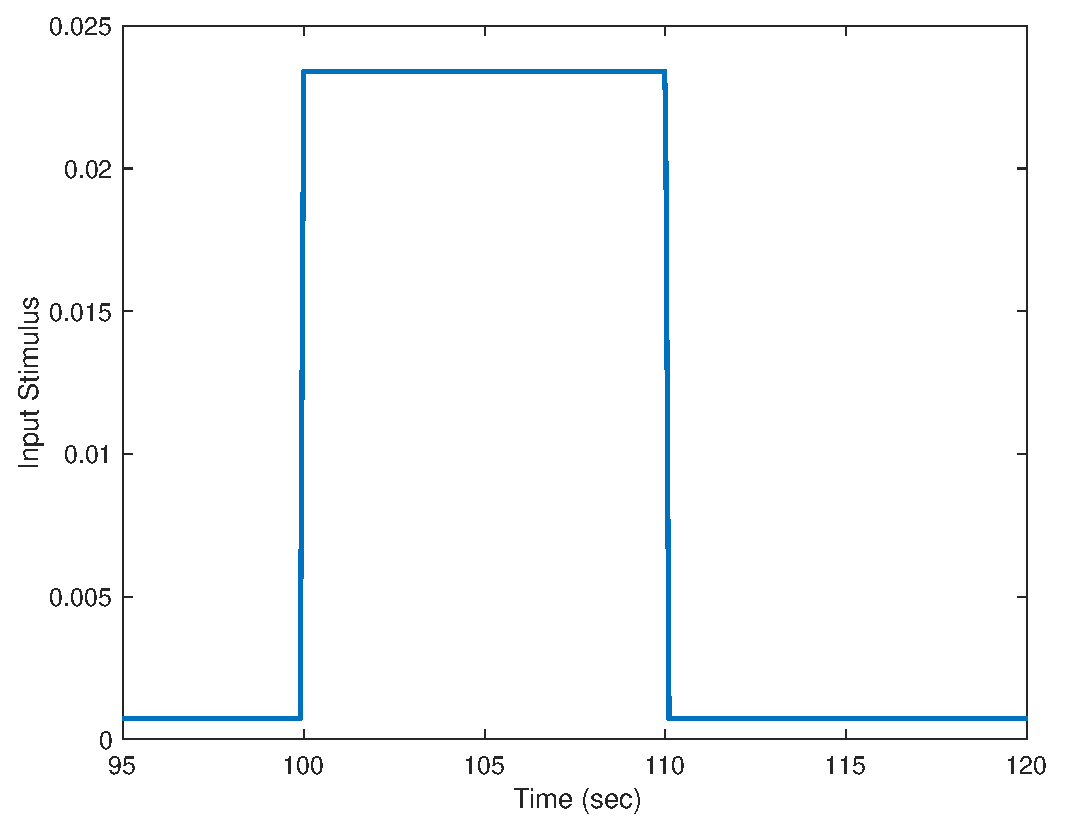
\includegraphics[width=.4 \textwidth]{Figures/Rectangular_Stimulus.eps}
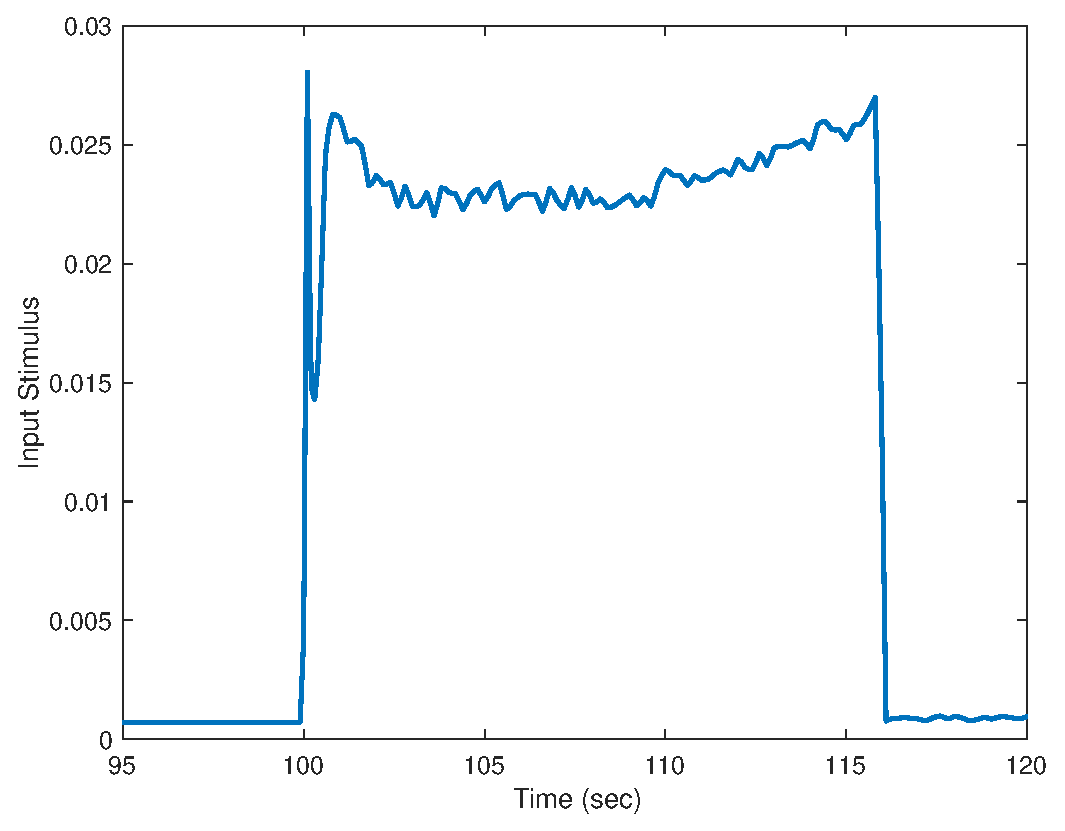
\includegraphics[width=.4 \textwidth]{Figures/Experimental_Stimulus.eps}
\caption{Left: rectangular pulse input stimulus; right: stimulus used in lab experiments.}
\label{input_stimuli}
\end{figure}
 Assuming the stimulation occurs for $t_1\le t \le t_2$, the QoIs are defined as follows.
\begin{enumerate}
\item ECS potassium has a distinct effect on the flux into the Neuron. Hence we look at the average.
\begin{eqnarray}
%[K^+]_{max,ECS} \label{K_ECS_Max} \\
 \frac{1}{t_2-t_1}\int_{t_1}^{t_2}[K^+]_{ECS}(s)ds \label{K_ECS_Mean}
\end{eqnarray}

\item As a representation of the volumetric flow rate in the cerebral tissue
\begin{equation}
\frac{1}{t_2-t_1}\int_{t_1}^{t_2}\left(\frac{R(s)}{R_0}\right)^4ds \label{vol_flow}
\end{equation}
 
%\item ECS potassium has a distinct effect on the flux into the astrocyte. Hence we look at the average and the maximum.
%\begin{eqnarray}
%[K^+]_{max,AC} \label{K_AC_Max} \\
%\frac{1}{t_2-t_1}\int_{t_1}^{t_2}[K^+]_{AC}(s)ds \label{K_AC_Mean}
%\end{eqnarray}
\item The combined concentration of the actin myosin complex, both phosphorylated and unphosphorylated, determines the effect stress due to the contraction for the smooth muscle cell. 
\begin{eqnarray}
[AM+AM_p]_{min} \label{AM_AMp_Min}
\end{eqnarray}

%\item The phase lag between neuronal stimulation and the radius changed effects a number of markers. Notably the BOLD signal, hence we choose to investigate
% the time, $\tau$, to min value of $AM_p$
% \begin{eqnarray}
% \tau = t_{min}-t_1 \label{AMp_Time_to_Min}
% \end{eqnarray}
\end{enumerate}

In addition, we consider the average concentration of AC potassium. It exhibits very small variation with respect to the parameters so we do not report any additional results for this QoI.

\subsection{Surrogate models and Sobol' indices}
There are a plurality of methods which may be used to analyse the sensitivity of a QoI to uncertain parameters. The large parameter dimension and computational cost of model evaluations prohibit many commonly used methods. A linear regression model of the form
\begin{eqnarray*}
\beta_0 + \sum\limits_{k=1}^{160} \beta_k \theta_k
\end{eqnarray*}
is fit to sample data (collected by running the model for various parameter samples) and the sensitivity of the linear model with respect to $\theta_k$ is defined as
\begin{eqnarray*}
L_k = \frac{\vert \beta_k \vert}{\sum\limits_{j=1}^{160} \vert \beta_j \vert}, \qquad k=1,2,\dots,160.
\end{eqnarray*}

In order to fit a nonlinear surrogate model, we reduce the parameter space to only the $\theta_k$'s such that $L_k>0.01$. Then a sparse Polynomial Chaos (PC) surrogate is fit using the sample data with the parameters $\{\theta_{k_i}\}_{i=1}^r$, where $L_{k_i}>0.01$, $i=1,2,\dots,r$. In Section~\ref{sec:results}, this reduction yields around $15-20$ parameters instead of the original 160. The PC surrogate is fit using the metamodel type \textit{PCE} in the UQLab \cite{uqlab}. The total Sobol' indices \cite{saltellitotalindex} of the PC surrogate are computed to yield a quantitative measure of importance for each $\theta_{k_i}$, $i=1,2,\dots,r$.

This procedure of 
\begin{enumerate}
\item[(i)] reducing dimension with linear regression,
\item[(ii)] fitting a Polynomial Chaos surrogate using the smaller set of parameters,
\item[(iii)] computing total Sobol' indices of the Polynomial Chaos surrogate,
\end{enumerate}
is used for each QoI considered in this article. All surrogate models are validated using 10-fold cross validation.

\section{Results}
\label{sec:results}
This section details our approach to varying the parameters and contains numerical results for the 3 QoI's, with both the square pulse stimulus and the experimental data stimulus for each. The section is organized in four subsections, one on the parameter sampling and one for each of the three QoI's.

\subsection{Parameter sampling}
\label{sec:param_sampling}
Distributions for the parameters are not known a priori, nor are they able to be estimated from experimental data. The subsection below details our computational approach to determine a distribution for the parameters. The computation time required for model evaluations with a stimulus applied is too great for the computational approach below. Rather, we focus on properties of the solution when no stimulus is applied, i.e. the steady state solution(s). This affords the needed computational acceleration. 

Parameter distributions are determined by first assuming independence of the parameters and assigning each parameter a uniform distribution with +- 10\% uncertainty around its nominal value (larger amounts of uncertainty may be desirable but are not computationally feasible). Parameters are likely to be correlated but we do not know the correlation structure a priori. The model is run, with no stimulus applied, for 919 different parameter samples. Of these 919 runs, 670 of them fail due to ode15s terminating prematurely because its time steps became too small. The remaining 249 yields 139 solutions which the radius reaches a stable steady state (at least for the duration of the time integration) and 110 solutions for which the radius reaches a steady state but subsequently because transient. The left panel of Figure~\ref{steady_states} displays four representative solutions for the radius; the red curves remain in steady state for the duration of our time integration whereas the black curves revert into a transit regime after some time in or near steady state. The right panel of Figure~\ref{steady_states} displays the samples for two parameters (in the buffer equation) which are highly influential in determining the behavior of the solution. A blue * indicates a sample where the solver terminated prematurely, a yellow + indicates a sample where an unstable steady state was observed, a red $\circ$ indicates a sample where the solution remained in steady state. A strong correlation determining the behavior of the solution is observed.

\begin{figure}[h]
\centering
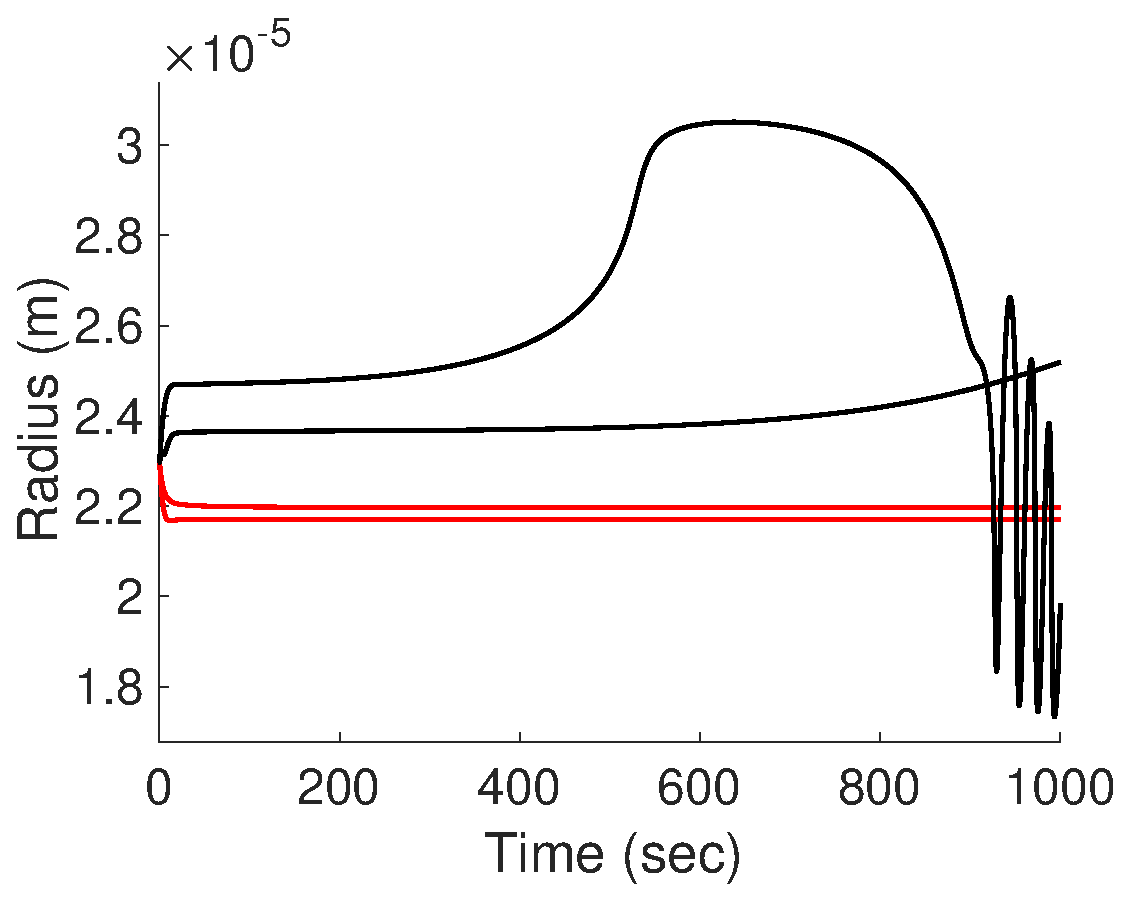
\includegraphics[width=.4 \textwidth]{Figures/Steady_State_Curves.eps}
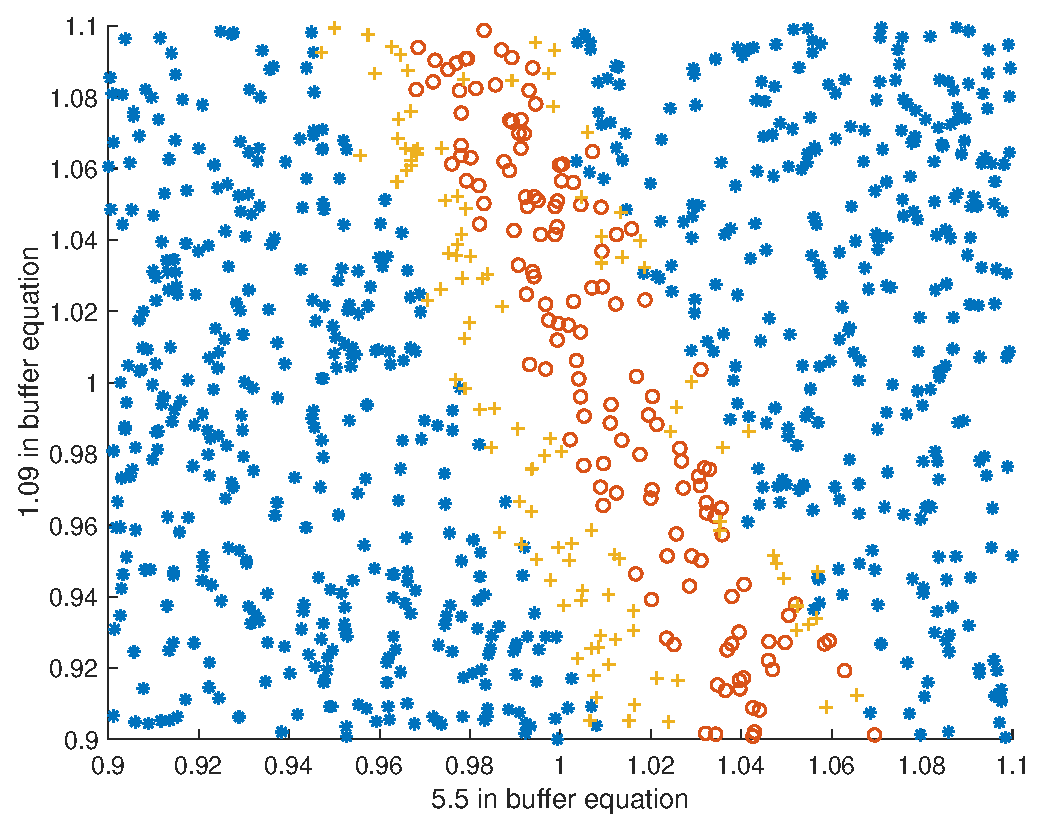
\includegraphics[width=.4 \textwidth]{Figures/First_Iteration_Samples.eps}
\caption{Left: examples of stable (red) and unstable (black) steady state solutions. Right: samples of the buffer parameters using uniform independent sampling. A blue \* indicates the sample yielded a premature termination of the solver, a yellow + indicates the sample yielded an unstable steady state, a red $\circ$ indicates the sample yielded a stable steady state.}
\label{steady_states}
\end{figure}

Observing this correlation, we use the samples for which the radius remained in steady state to fit the two buffer parameters with a bivariate distribution with beta marginals and a Frank copula. The experiment was repeat by sampling the two correlated parameters with the bivariate distribution and all other parameter from their original uniform distributions. The samples yielding steady state solutions where collected, a bivariate distribution fit to them, and the experimented was repeated. After three additional iterations of this process we were able to generate 902 out of 960 samples which yielded solutions with stable steady states (51 solutions had unstable steady states and 7 had premature solver terminations). This fitted distribution is used for all subsequent analysis. 

Samples are drawn and the model, with a stimulus applied (in two separate cases, the 10 second rectangular pulse and the 16 second stimulus from experimental data), is run for each sample. This results in solutions exhibiting three different physiological regimes; they are displayed in Figure~\ref{solution_regimes} where the radius is plotted as a function of time. The leftmost panel corresponds to the typical case when the radius increases in response to the stimulus and then decreases when it is removed; the center panel corresponds to an atypical case where the radius has an initial decrease in response to the stimulus; the right panel corresponds to another atypical case where the radius reaches another steady state an does not decrease after the stimulus is removed.

\begin{figure}[h]
\centering
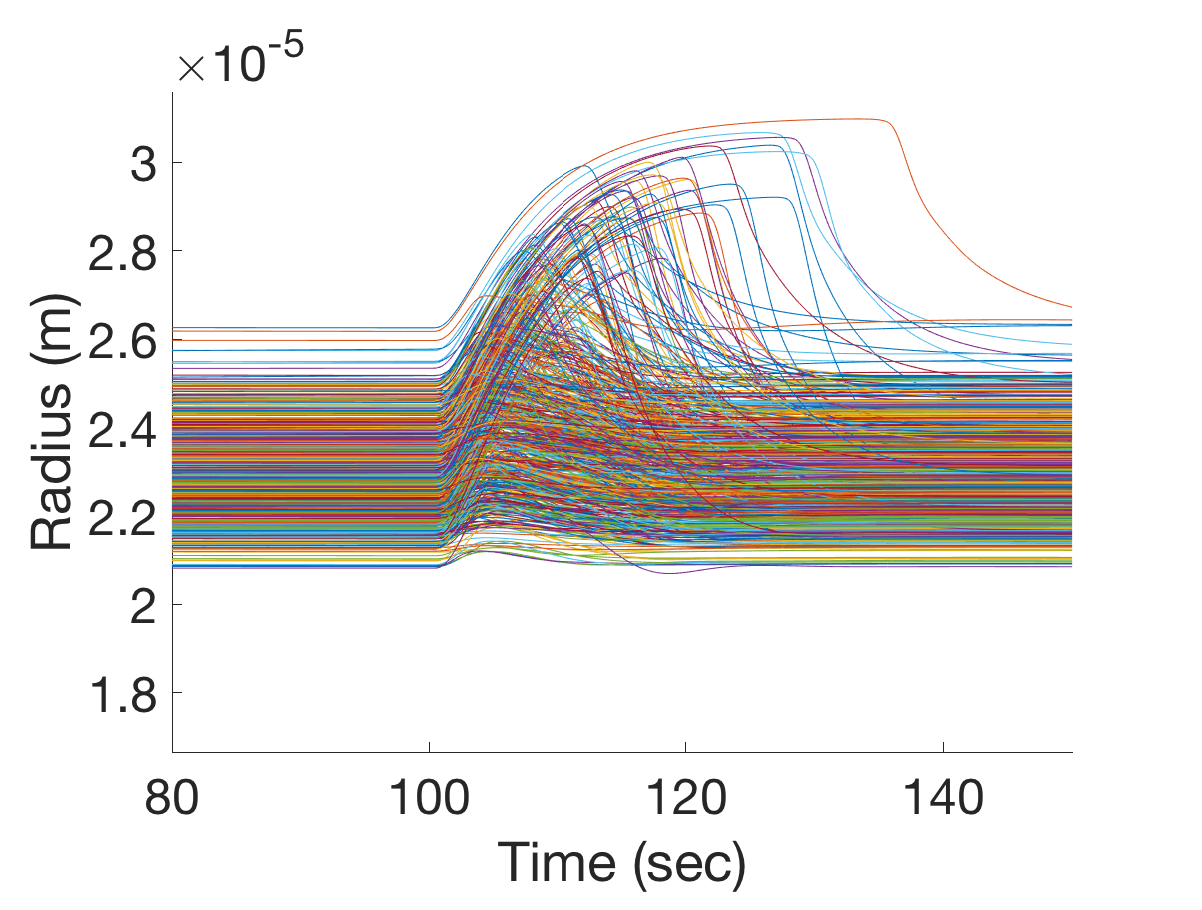
\includegraphics[width=.3 \textwidth]{Figures/Increase_with_Stim_Curves.eps}
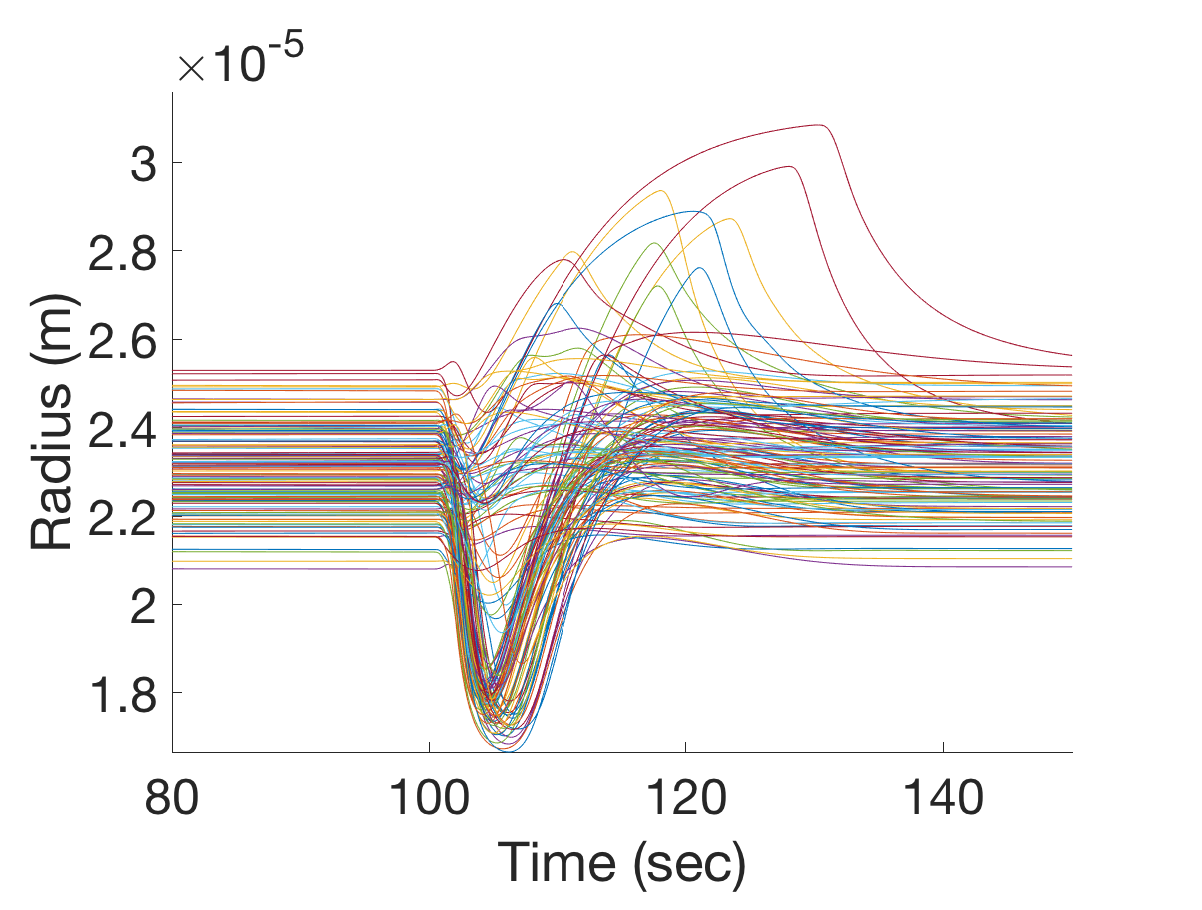
\includegraphics[width=.3 \textwidth]{Figures/Decrease_with_Stim_Curves.eps}
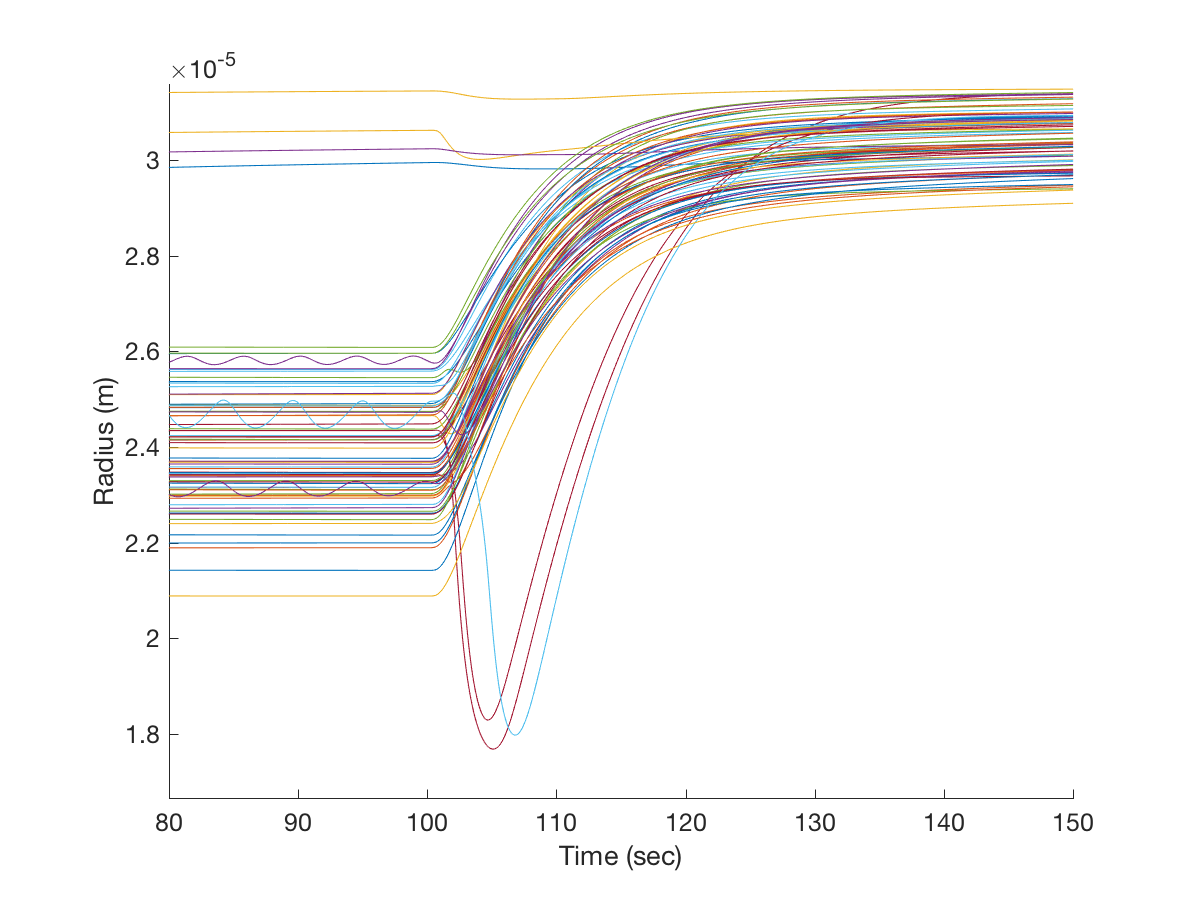
\includegraphics[width=.3 \textwidth]{Figures/Higher_Steady_State.eps}
\caption{Radii corresponding to samples (using the rectangular pulse stimulus). Left: curves an an increase in response to the stimulus; center: curves with a decrease in response to the stimulus; right: curves which settle in a different steady state.}
\label{solution_regimes}
\end{figure}

This article focuses on the typical case so we remove samples where the radius does not increase in response to the stimulus and decrease when it is removed. This processing yields 660 samples for analysis when the rectangular pulse stimulus is applied and 438 samples when the stimulus from experimental data is applied. The results presented below use these samples.

Exploration of the 660 retained samples indicate that atypical cases have higher probability when the parameter 34.9 in m2alpha is small; however, this parameter does not characterize the solution regime by itself; it is likely that the solution regime is characterized by a combination of several parameters. Further sampling and exploration is required to better understand the structure in parameter space which determine the solution regime.

\subsection{QoI \eqref{K_ECS_Mean} ($K_{ECS}$ Mean)}
\label{sec:qoi_K_ECS_Mean}

Figure~\ref{fig:K_ECS_Mean} displays results for the average of the ECS potassium. Across the top and bottom rows we present results for the rectangular pulse stimulus and experimental data stimulus, respectively. In the leftmost panel, predictions of the linear regression surrogate are plotted against the model values. The sensitivities $L_k$, $k=1,2,\dots,160$, are displayed in the center-left panel. Predictions of the PC surrogate are plotted against the model values in the center-right panel. The total Sobol' indices of the PC surrogate are given in the rightmost panel. Table~\ref{tab:K_ECS_Mean} reports the 5 most important parameters and their total Sobol' indices.

\begin{figure}[h]
\centering
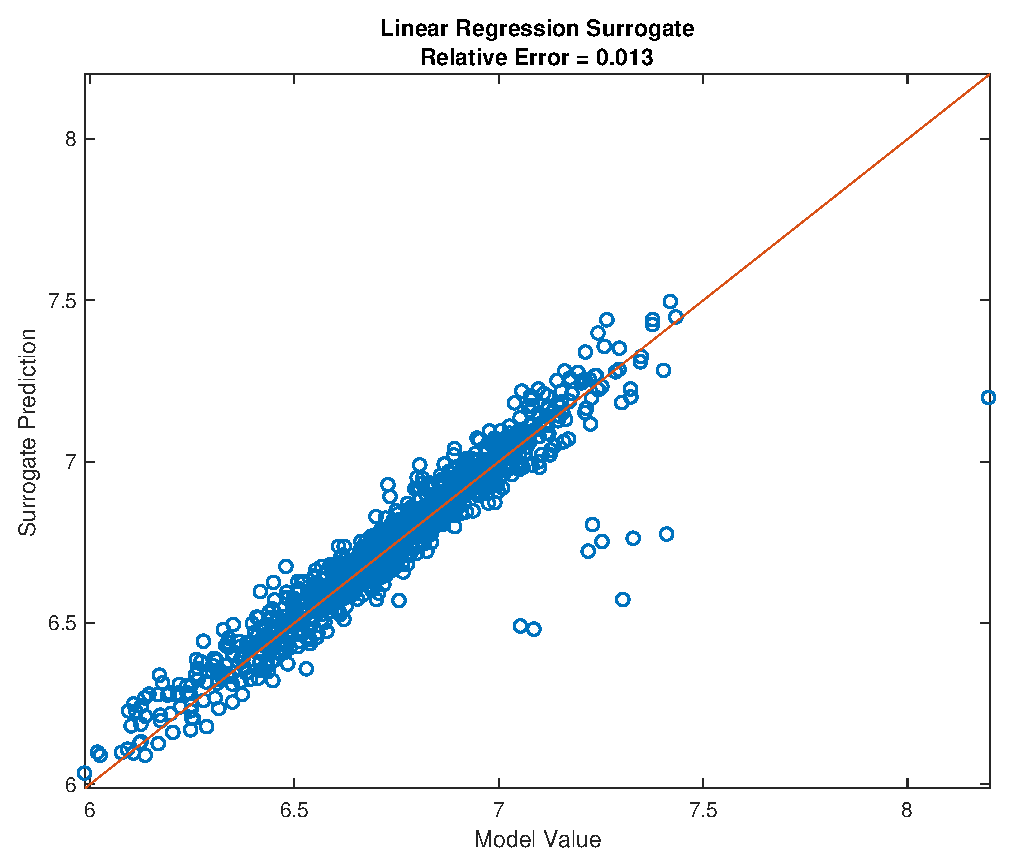
\includegraphics[width=.24 \textwidth]{Figures/K_ECS_Mean_QoI_LR_Prediction_Rectangular.eps}
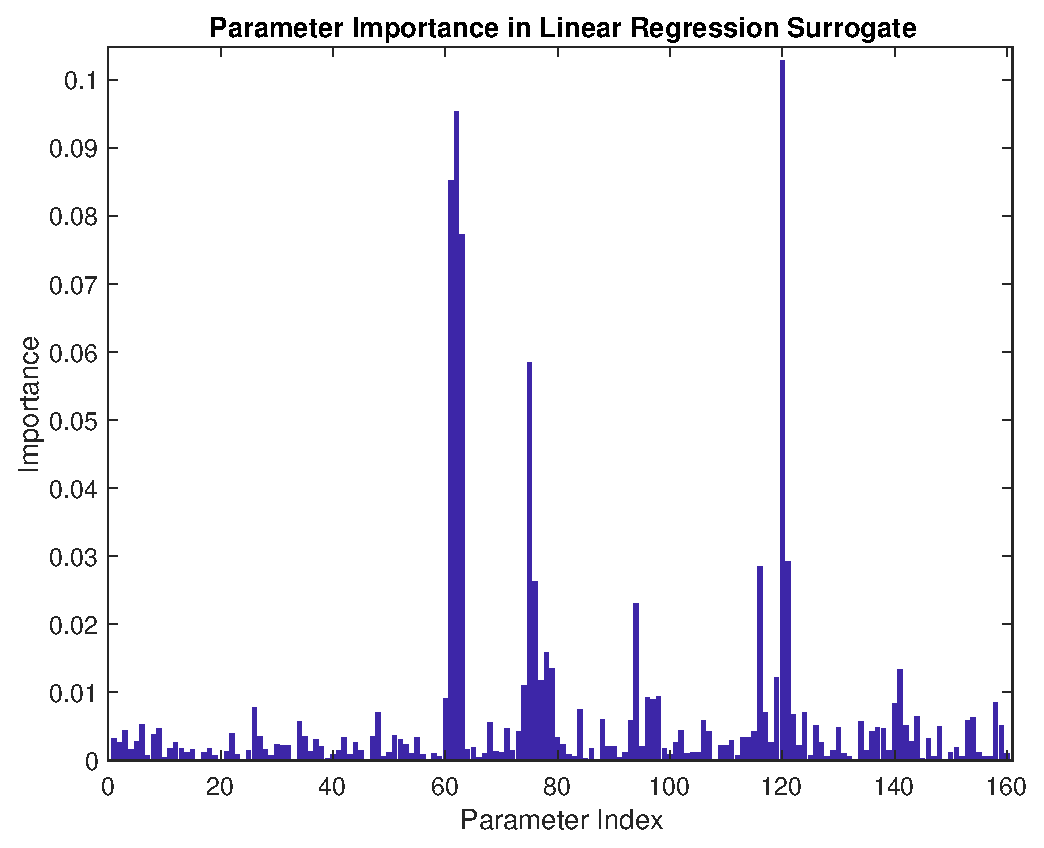
\includegraphics[width=.24 \textwidth]{Figures/K_ECS_Mean_QoI_LR_VI_Rectangular.eps}
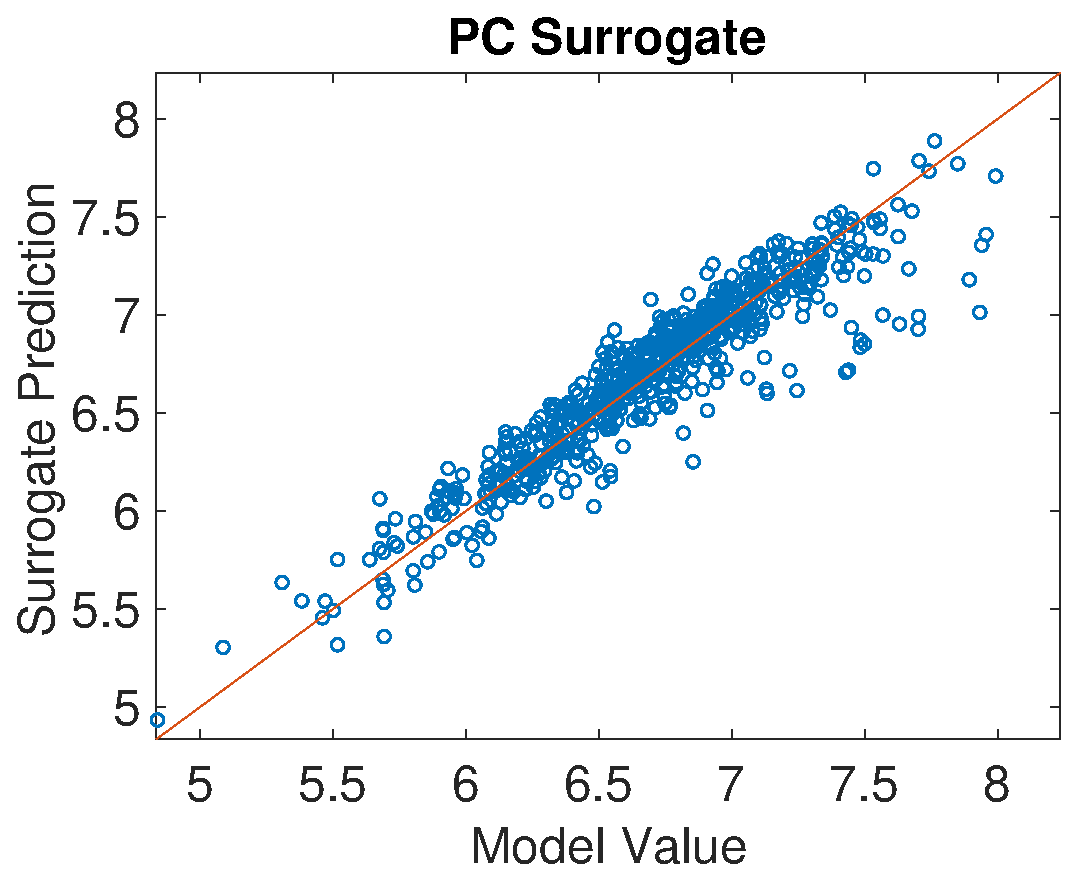
\includegraphics[width=.24 \textwidth]{Figures/K_ECS_Mean_QoI_PCE_Prediction_Rectangular.eps}
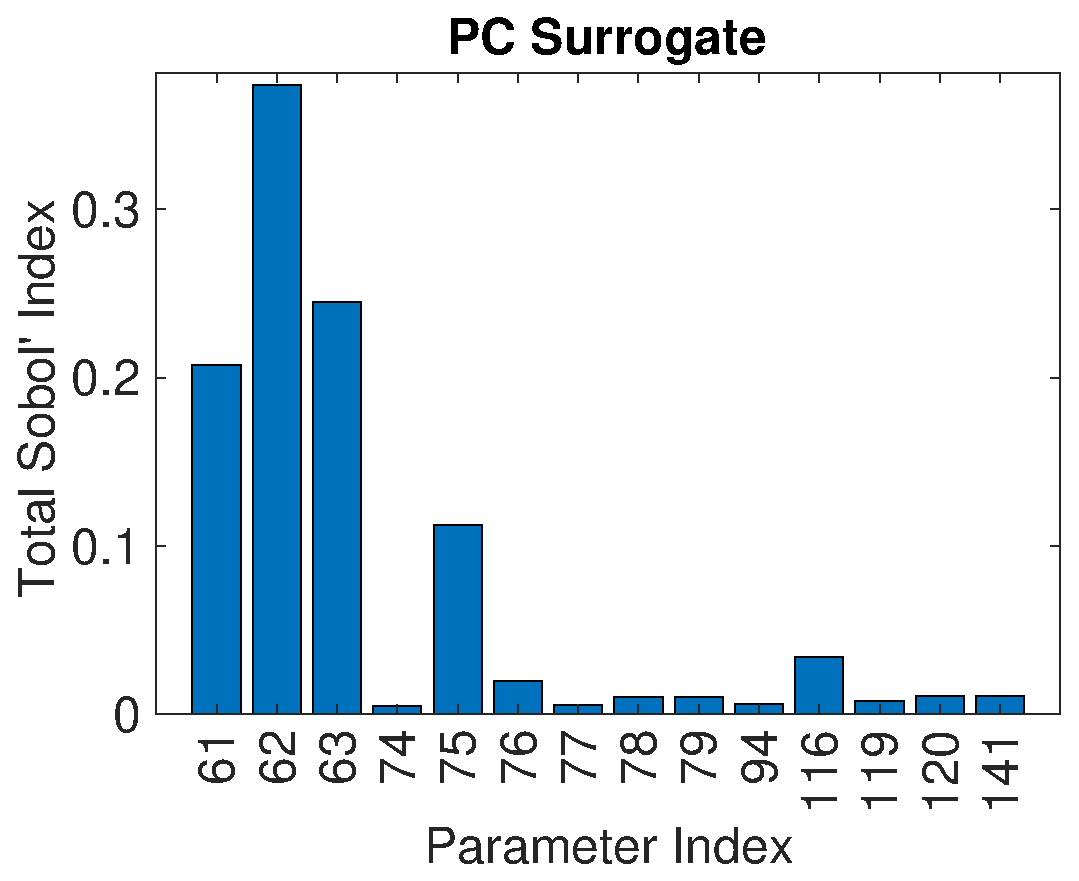
\includegraphics[width=.24 \textwidth]{Figures/K_ECS_Mean_QoI_PCE_SI_Rectangular.eps}\\
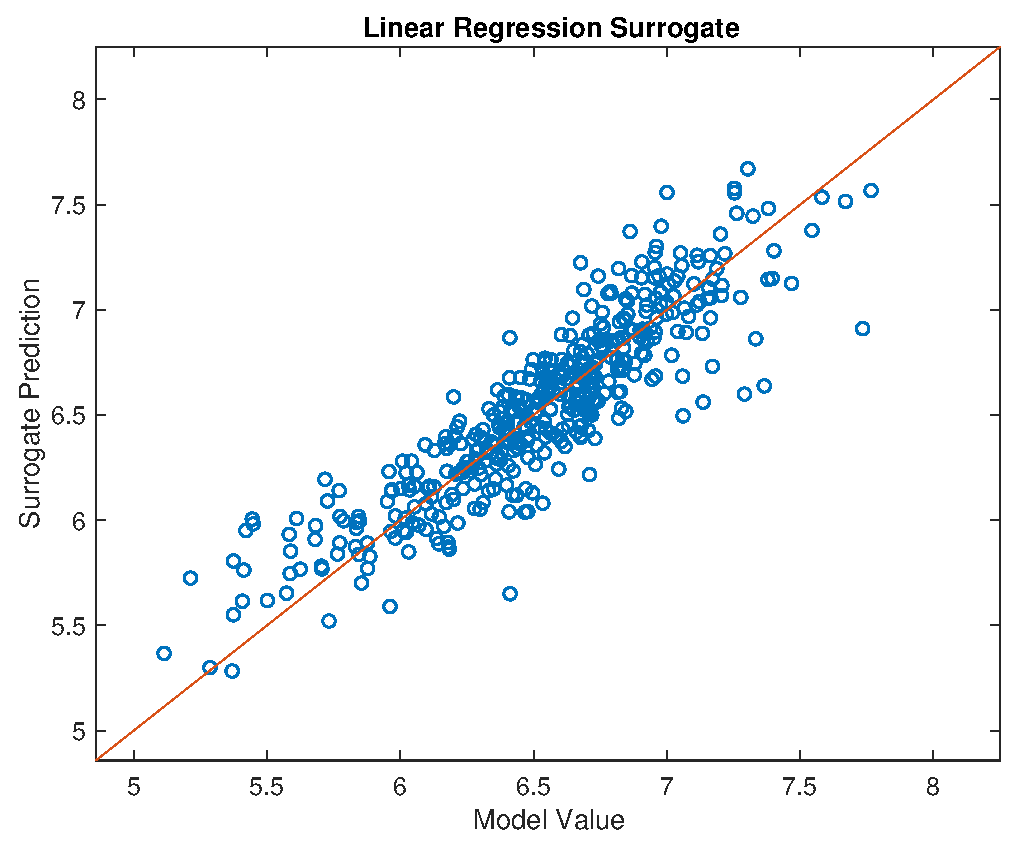
\includegraphics[width=.24 \textwidth]{Figures/K_ECS_Mean_QoI_LR_Prediction_Experimental.eps}
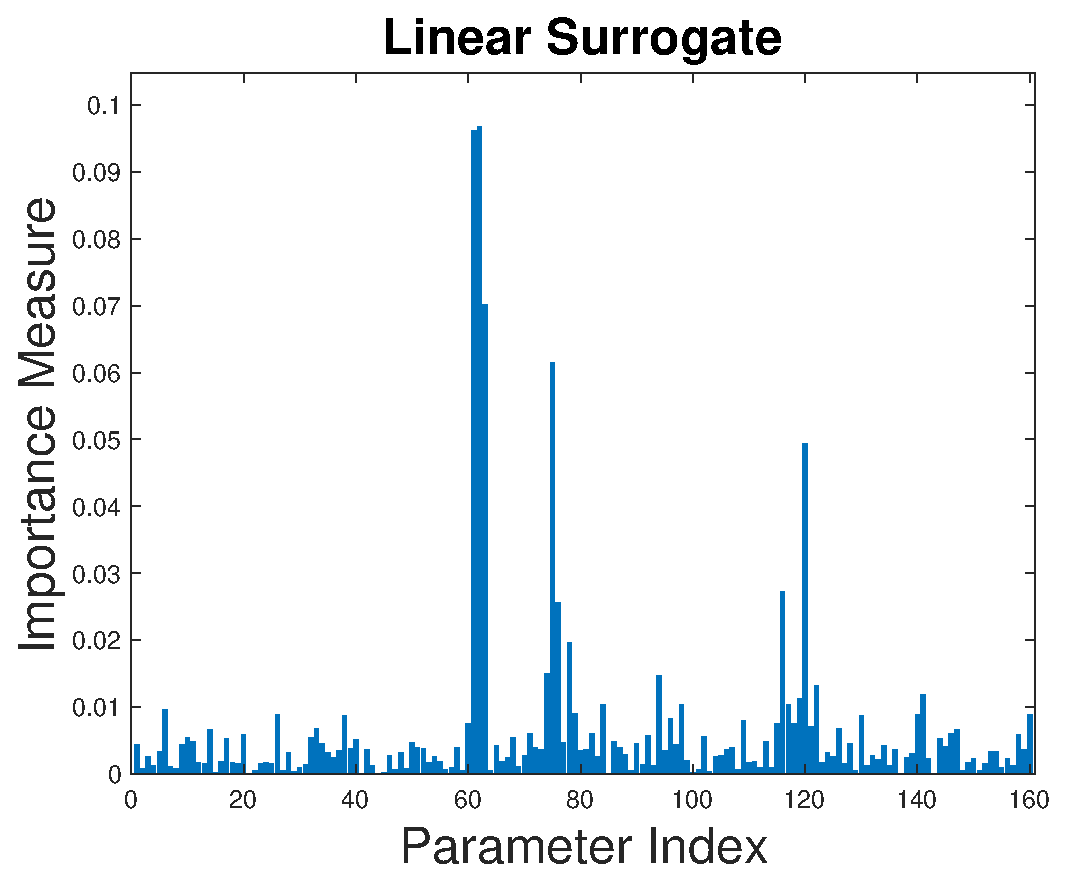
\includegraphics[width=.24 \textwidth]{Figures/K_ECS_Mean_QoI_LR_VI_Experimental.eps}
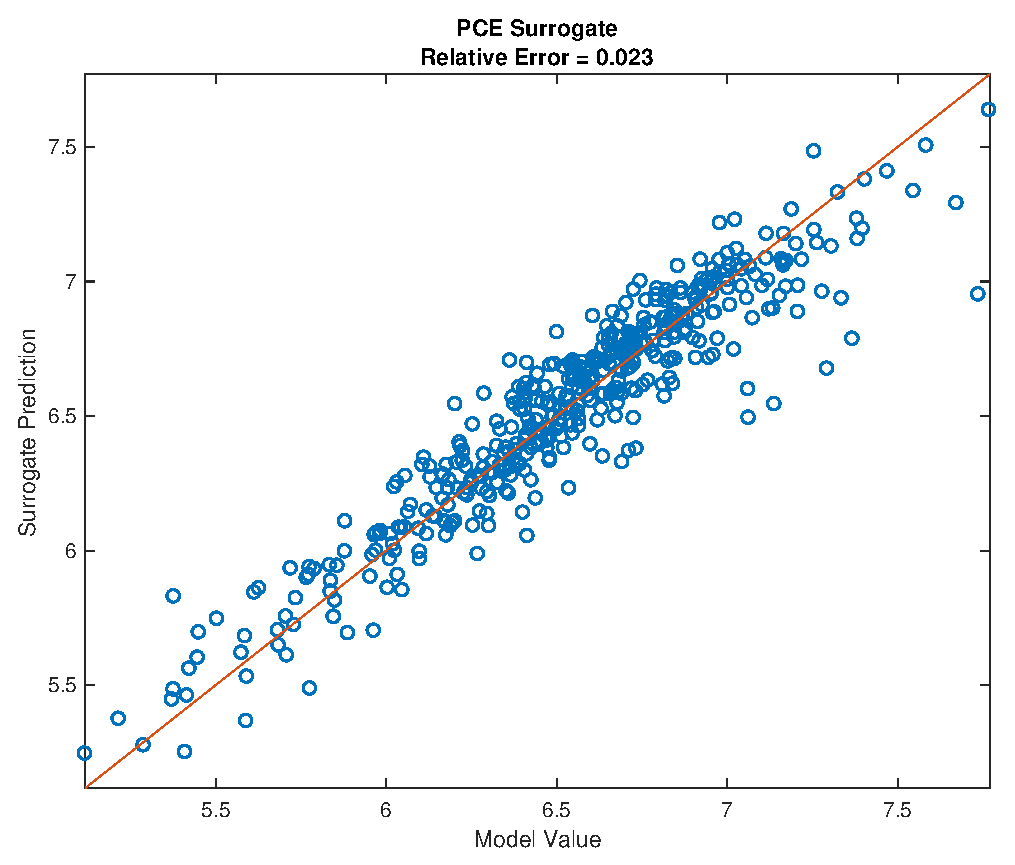
\includegraphics[width=.24 \textwidth]{Figures/K_ECS_Mean_QoI_PCE_Prediction_Experimental.eps}
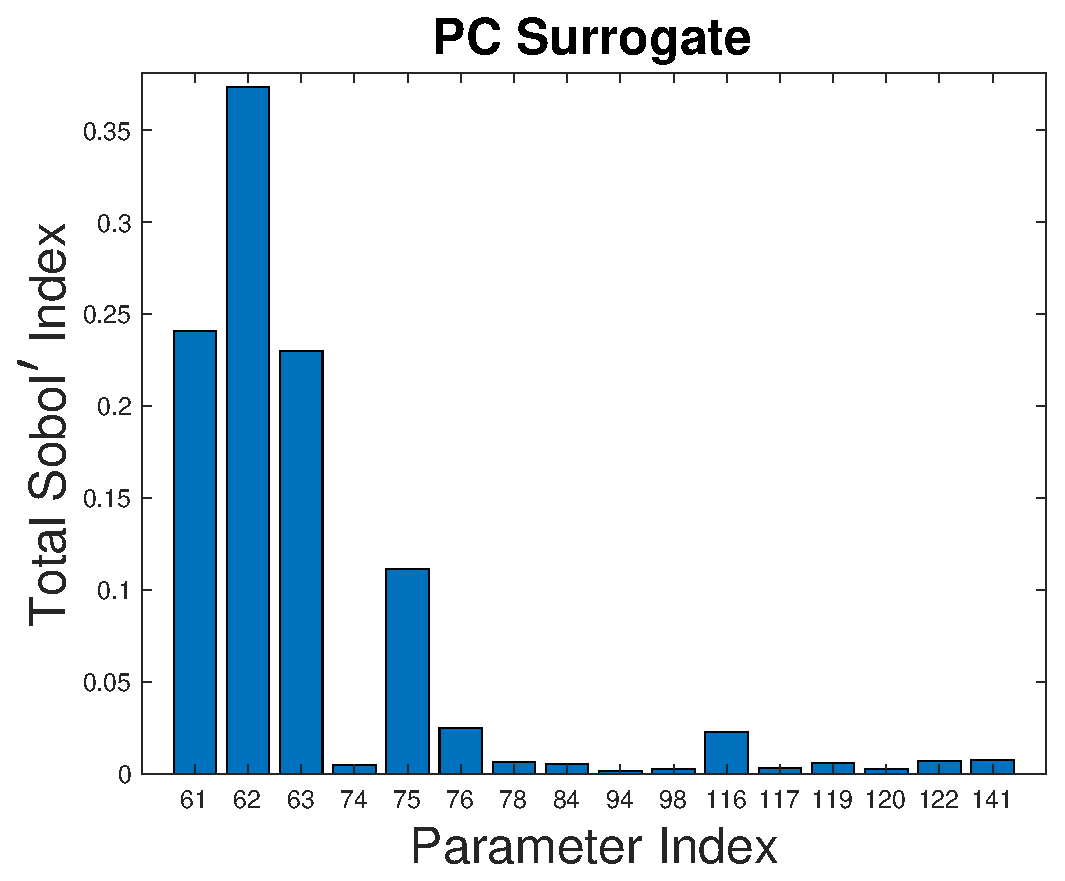
\includegraphics[width=.24 \textwidth]{Figures/K_ECS_Mean_QoI_PCE_SI_Experimental.eps}
\caption{Results for ECS potassium QoI. Top row: results with a rectangular pulse stimulus; bottom row: results with experimental data stimulus. From left to right, linear regression predictions, linear regression variable importance, PCE predictions, total Sobol' indices for PCE.}
\label{fig:K_ECS_Mean}
\end{figure}

\begin{table}[h]
\centering
\begin{tabular}{cccc}
Index & Identification & Total Sobol' Index (RP) & Total Sobol' Index (ES)\\
62 & 0.143 in m4alpha and m4 beta &  0.3744 & 0.3683\\
63 & 5.67 in m4alpha and m4 beta & 0.2446 & 0.2307\\
61 & gKleak\_d in Neuron & 0.2025 & 0.2485\\
75 & 34.9 in m6alpha & 0.1217 & 0.1070\\
116 & dhod in Neuron &  0.0348 & 0.0257\\
\end{tabular}
\caption{Most influential parameters for the ECS potassium QoI.}
\label{tab:K_ECS_Mean}
\end{table}

The results are similar for both the rectangular pulse and experimental data stimulus. In both cases, the QoI is approximated with reasonable accuracy by a linear model and with higher accuracy by the PC model. The most important parameters are shared in both cases. Notice that parameter 120 appears to be important in the linear model but unimportant in the PC model. This is because it is strongly correlated with parameter 121, see Figure~\ref{steady_states} and the discussion in Subsection~\ref{sec:param_sampling}, and as a result the coefficient in linear regression may be very large because its effect is offset by the effect of parameter 121. To decorrelate inputs, the PC surrogate is build with only parameter 120 instead of both 120 and 121. It subsequently has minimal importance.

\subsection{QoI \eqref{vol_flow} (volumetric flow rate)}

Figure~\ref{fig:qoi_vol_flow} displays results for the volumetric flow rate in the cerebral tissue. In the same manner as Figure~\ref{fig:K_ECS_Mean}, the linear and PC surrogate predictions and sensitivities are plotted for both the rectangular pulse and experimental data stimulus. Table~\ref{tab:qoi_vol_flow} reports the 5 most important parameters and their total Sobol' indices.

\begin{figure}[h]
\centering
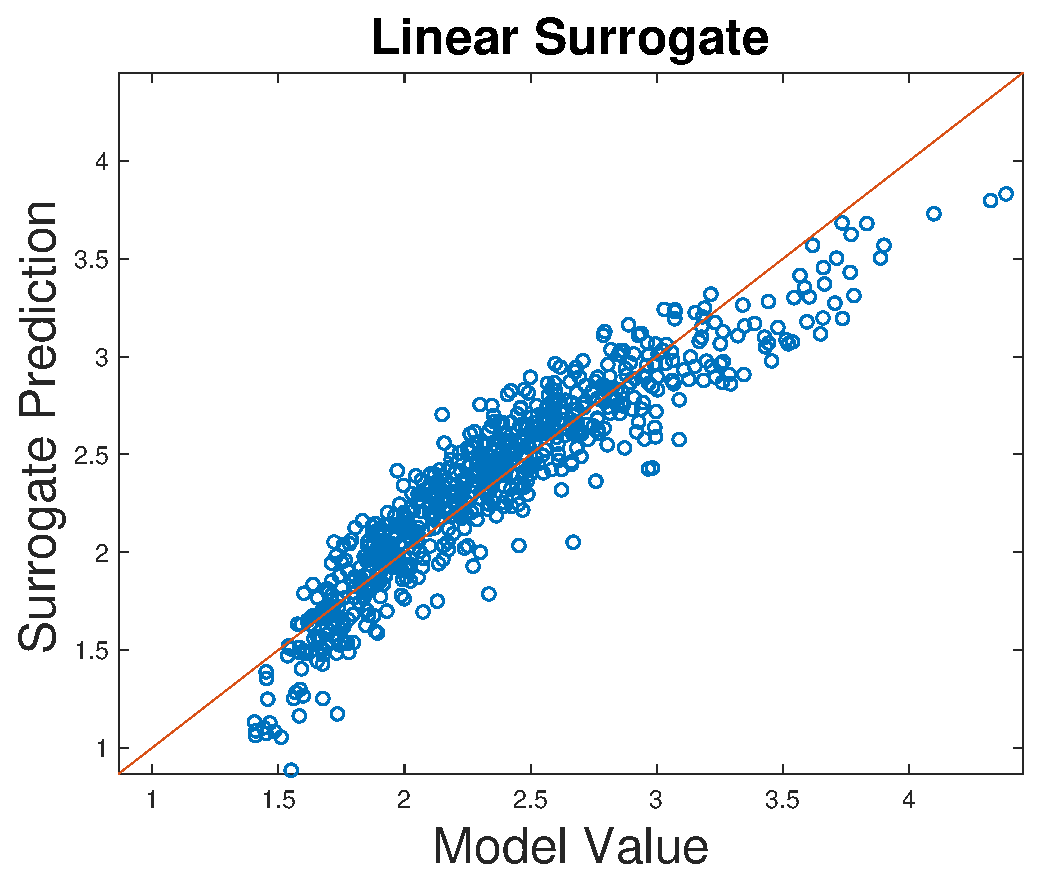
\includegraphics[width=.24 \textwidth]{Figures/Vol_Flow_QoI_LR_Prediction_Rectangular.eps}
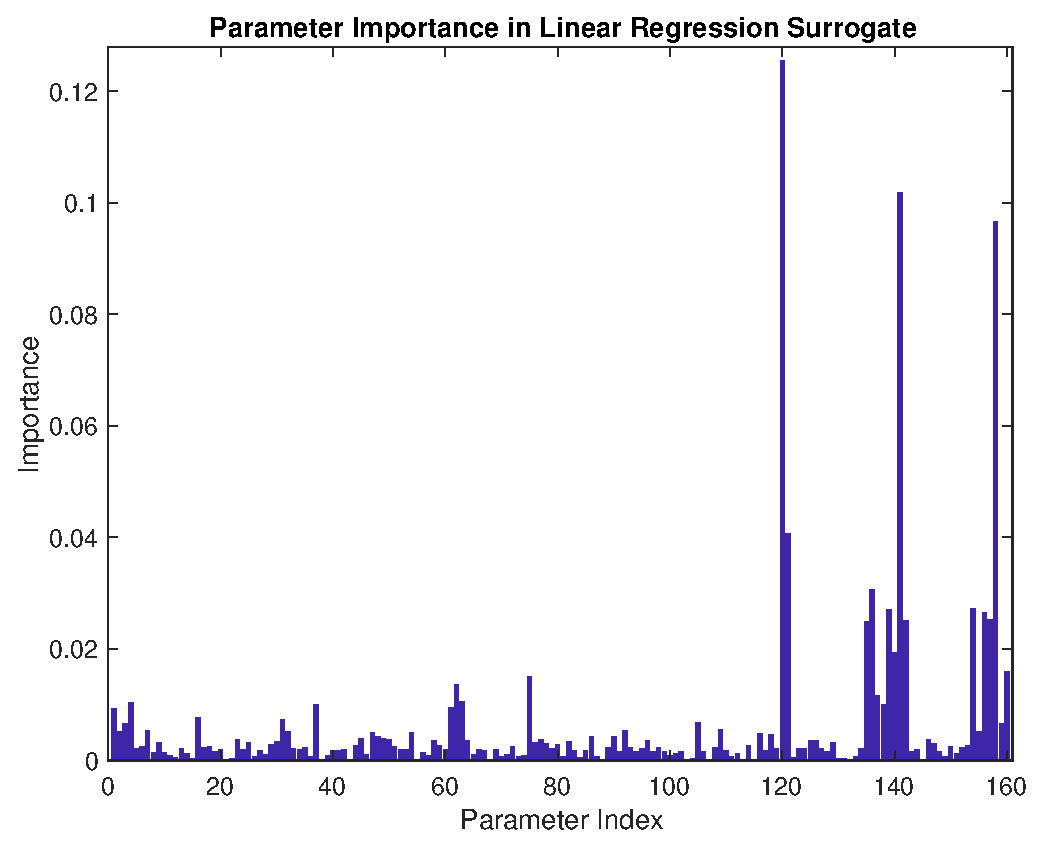
\includegraphics[width=.24 \textwidth]{Figures/Vol_Flow_QoI_LR_VI_Rectangular.eps}
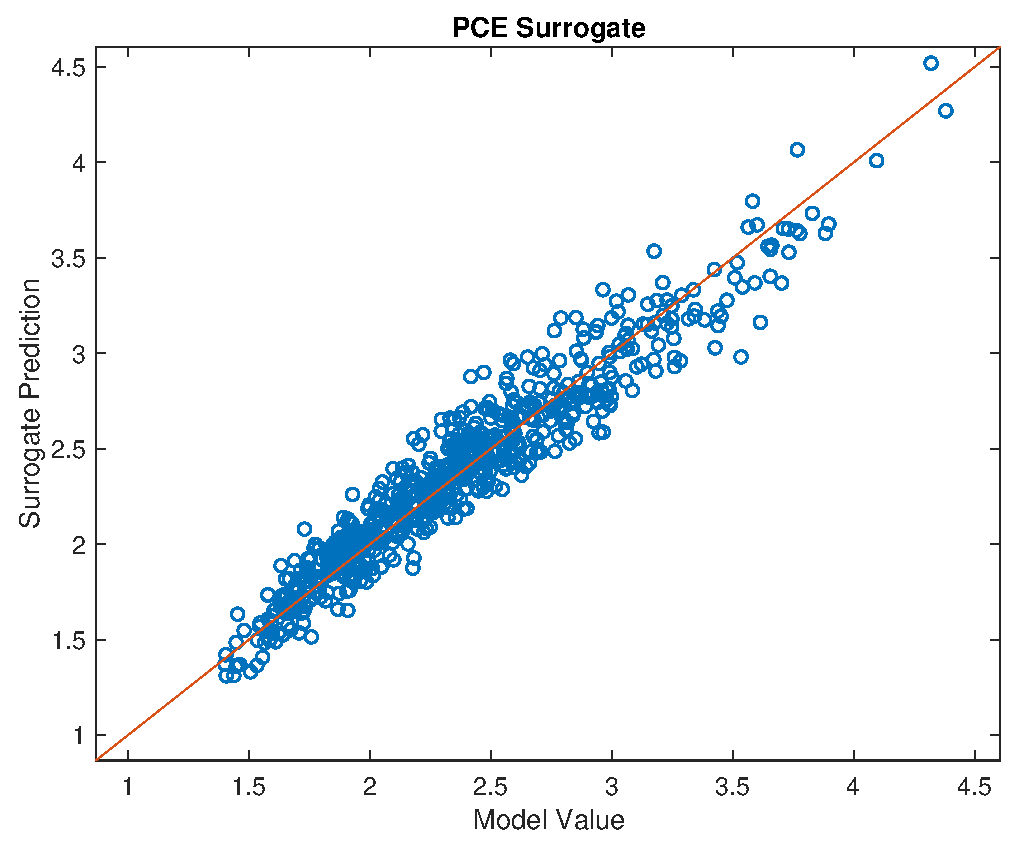
\includegraphics[width=.24 \textwidth]{Figures/Vol_Flow_QoI_PCE_Prediction_Rectangular.eps}
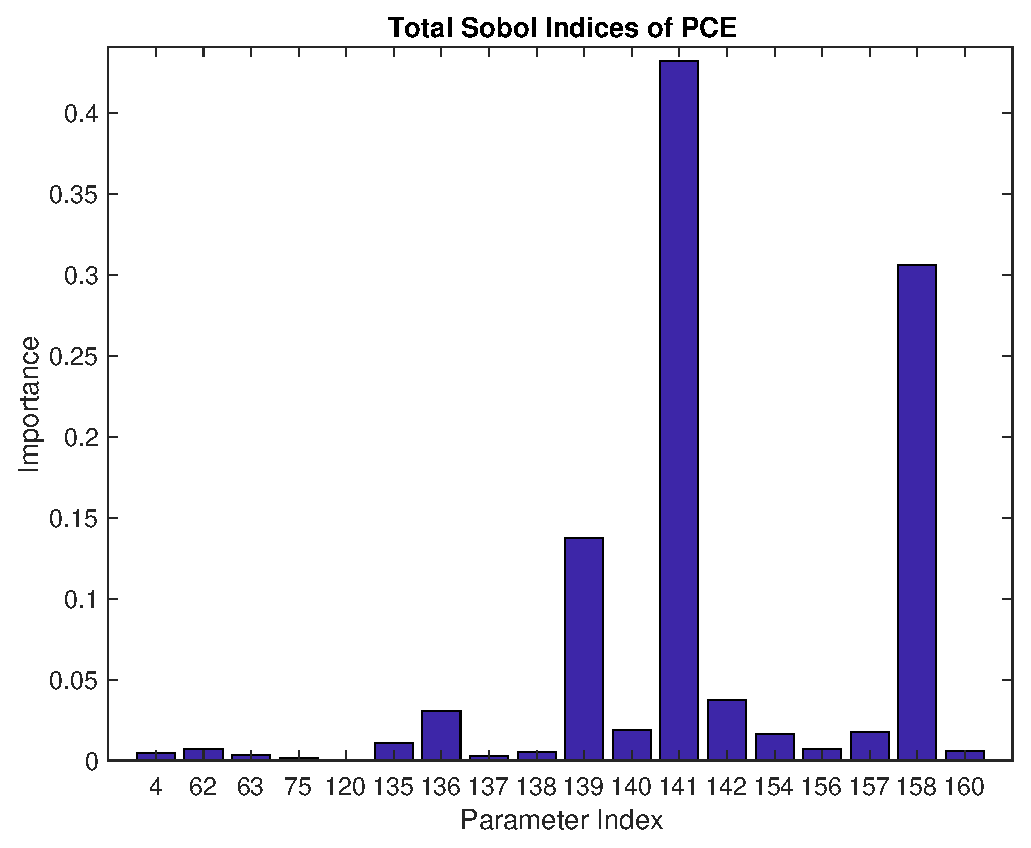
\includegraphics[width=.24 \textwidth]{Figures/Vol_Flow_QoI_PCE_SI_Rectangular.eps}\\
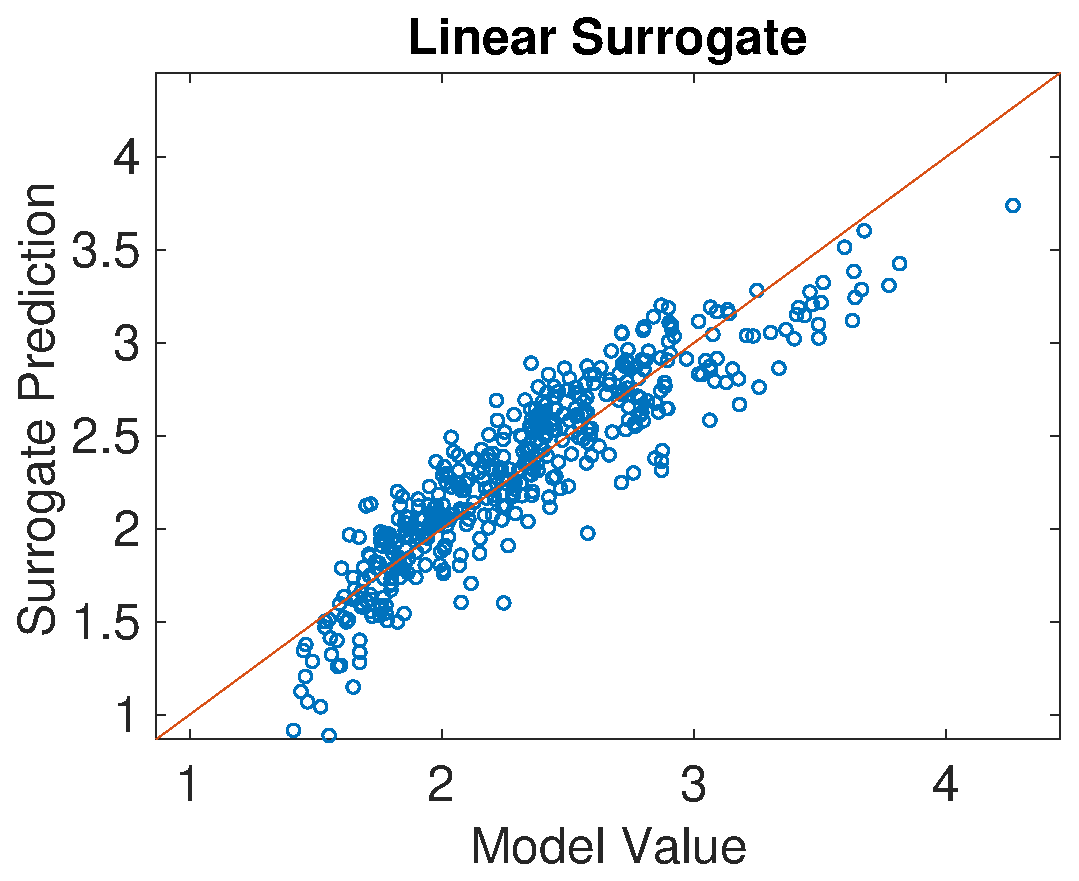
\includegraphics[width=.24 \textwidth]{Figures/Vol_Flow_QoI_LR_Prediction_Experimental.eps}
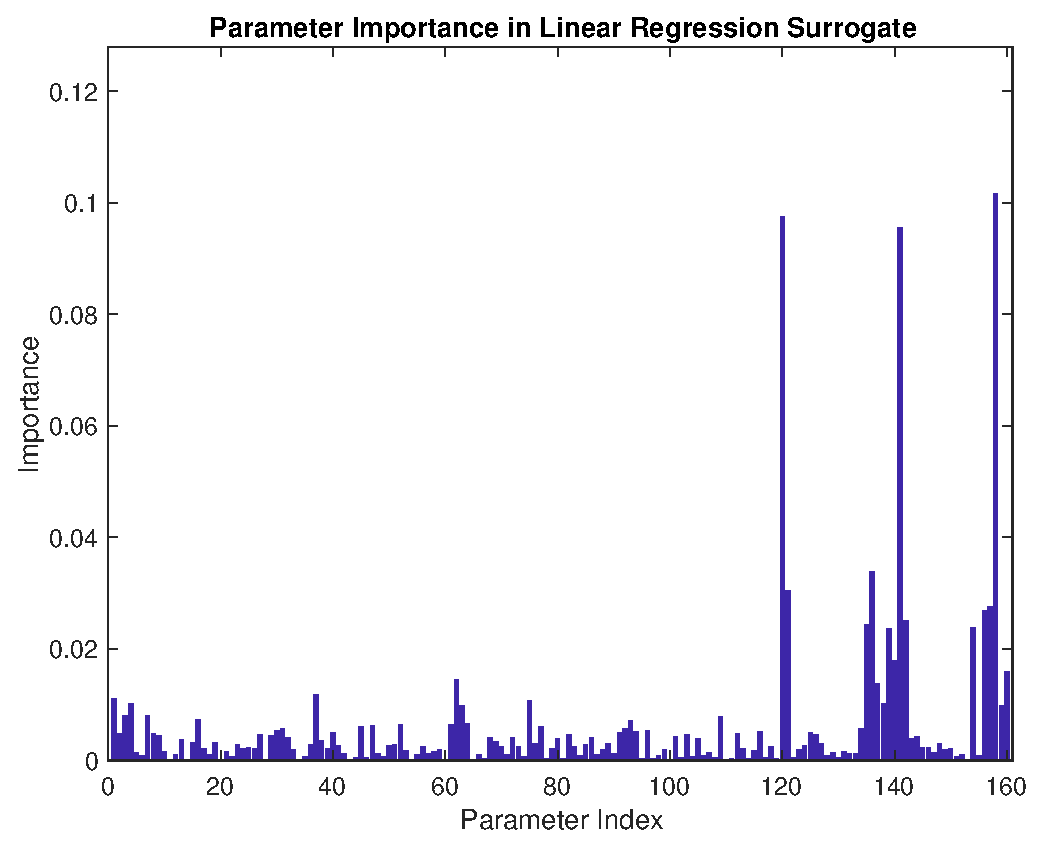
\includegraphics[width=.24 \textwidth]{Figures/Vol_Flow_QoI_LR_VI_Experimental.eps}
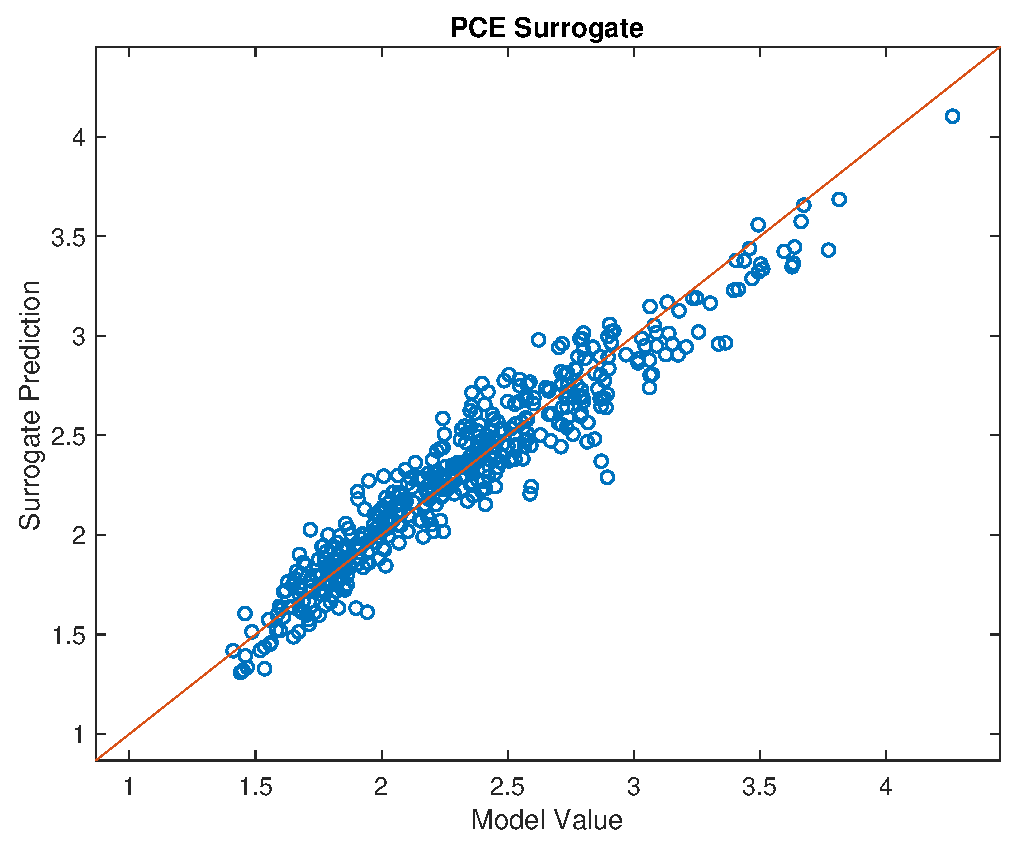
\includegraphics[width=.24 \textwidth]{Figures/Vol_Flow_QoI_PCE_Prediction_Experimental.eps}
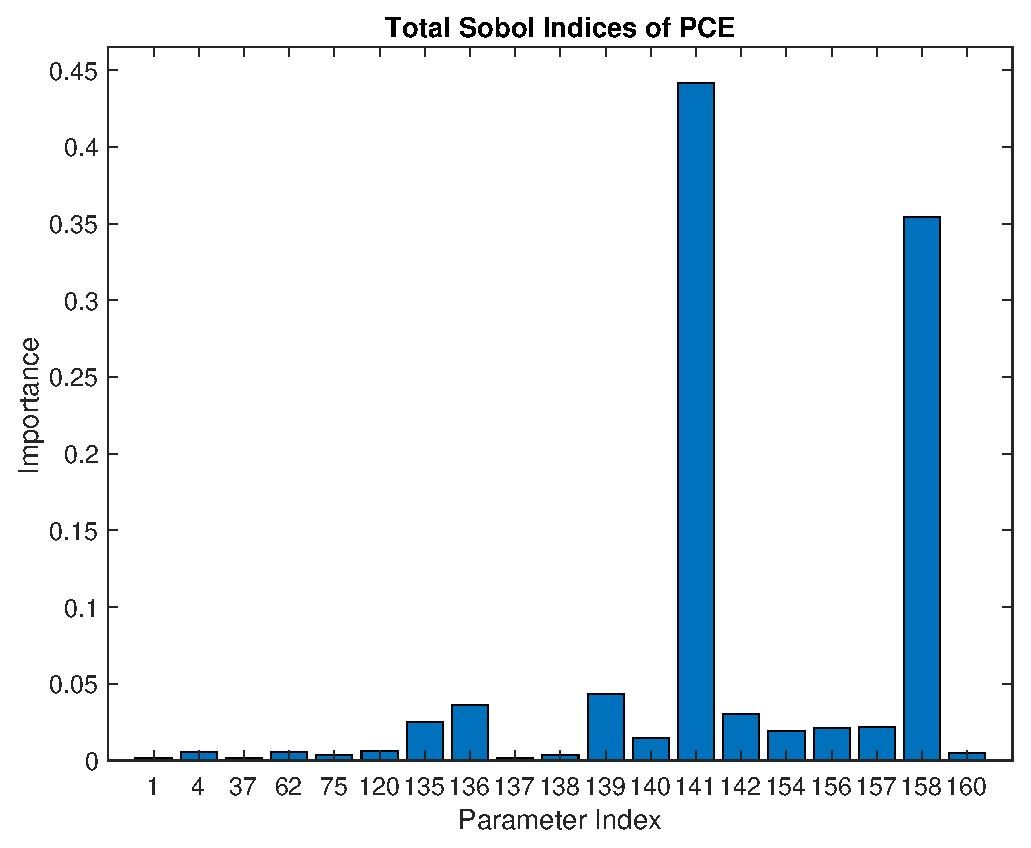
\includegraphics[width=.24 \textwidth]{Figures/Vol_Flow_QoI_PCE_SI_Experimental.eps}
\caption{Results for the volumetric flow rate in the cerebral tissue QoI. Top row: results with a rectangular pulse stimulus; bottom row: results with experimental data stimulus. From left to right, linear regression predictions, linear regression variable importance, PCE predictions, total Sobol' indices for PCE.}
\label{fig:qoi_vol_flow}
\end{figure}

We again observe reasonably accurate fits by a linear surrogate and improved accuracy by a PC surrogate. The surrogate predictions and important parameters for the rectangular pulse and experimental stimulus closely agree. The influential parameters for the volumetric flow rate in the cerebral tissue are different than those found to be influential for the ECS potassium. This is an unsurprising result. As in Subsection~\ref{sec:qoi_K_ECS_Mean}, parameter 120 appears important in the linear surrogate but unimportant in the PC surrogate.

\begin{table}[h]
\centering
\begin{tabular}{cccc}
Index & Identification & Total Sobol' Index (RP) & Total Sobol' Index (ES)\\
141 &  z\_4 in SMCEC &  0.4353 & 0.4445\\
158 & n\_cross in WallMechanics & 0.3045 & 0.3398\\
 139 & z\_2 in SMCEC & 0.1267 & 0.0478\\
 142 & z\_5 in SMCEC & 0.0347 & 0.0347\\
  136 & G\_K\_i in SMCEC & 0.0302 & 0.0359\\
\end{tabular}
\caption{Most influential parameters for the volumetric flow rate in the cerebral tissue QoI.}
\label{tab:qoi_vol_flow}
\end{table}

\subsection{QoI \eqref{AM_AMp_Min} ($AM+AM_p$ Min)}

Figure~\ref{fig:qoi_AM_AMp_Min} displays results for the minimum of the combined concentration of the actin myosin complex. As in the previous subsections, the linear and PC surrogate predictions and sensitivities are plotted for both the rectangular pulse and experimental data stimulus. Table~\ref{tab:qoi_AM_AMp_Min} reports the 5 most important parameters (ranked by the total Sobol' indices for the rectangular pulse stimulus) and their total Sobol' indices.

\begin{figure}[h]
\centering
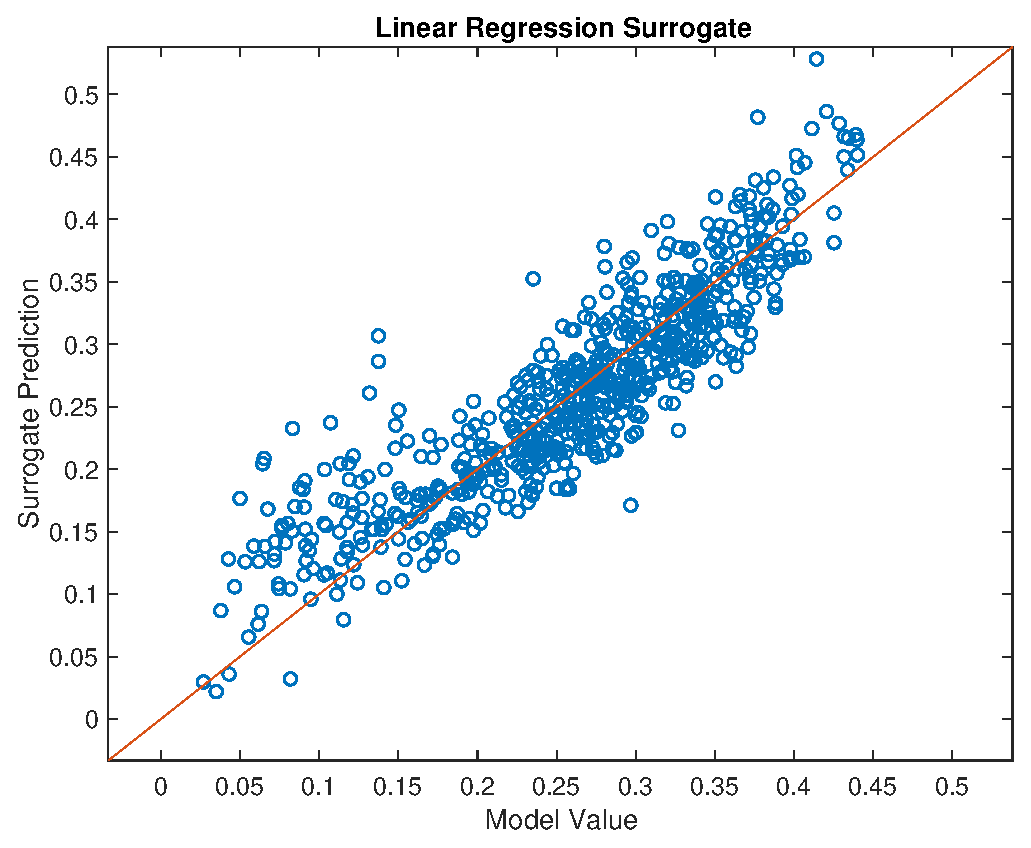
\includegraphics[width=.24 \textwidth]{Figures/AM_AMp_Min_QoI_LR_Prediction_Rectangular.eps}
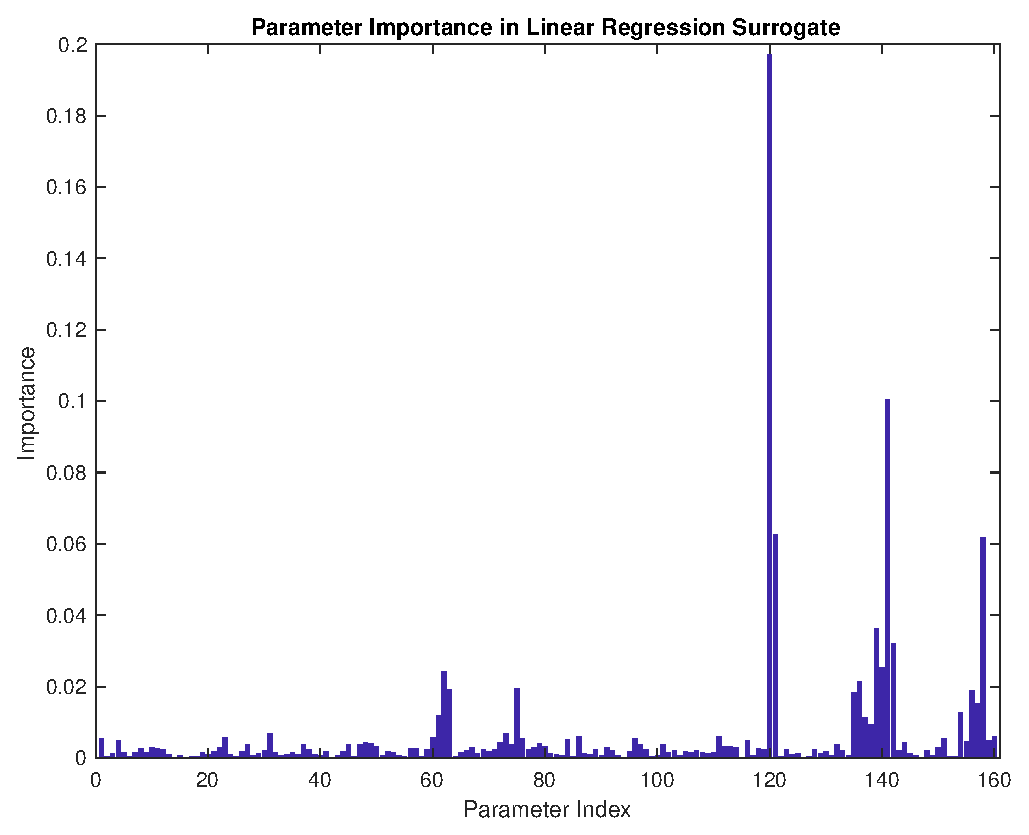
\includegraphics[width=.24 \textwidth]{Figures/AM_AMp_Min_QoI_LR_VI_Rectangular.eps}
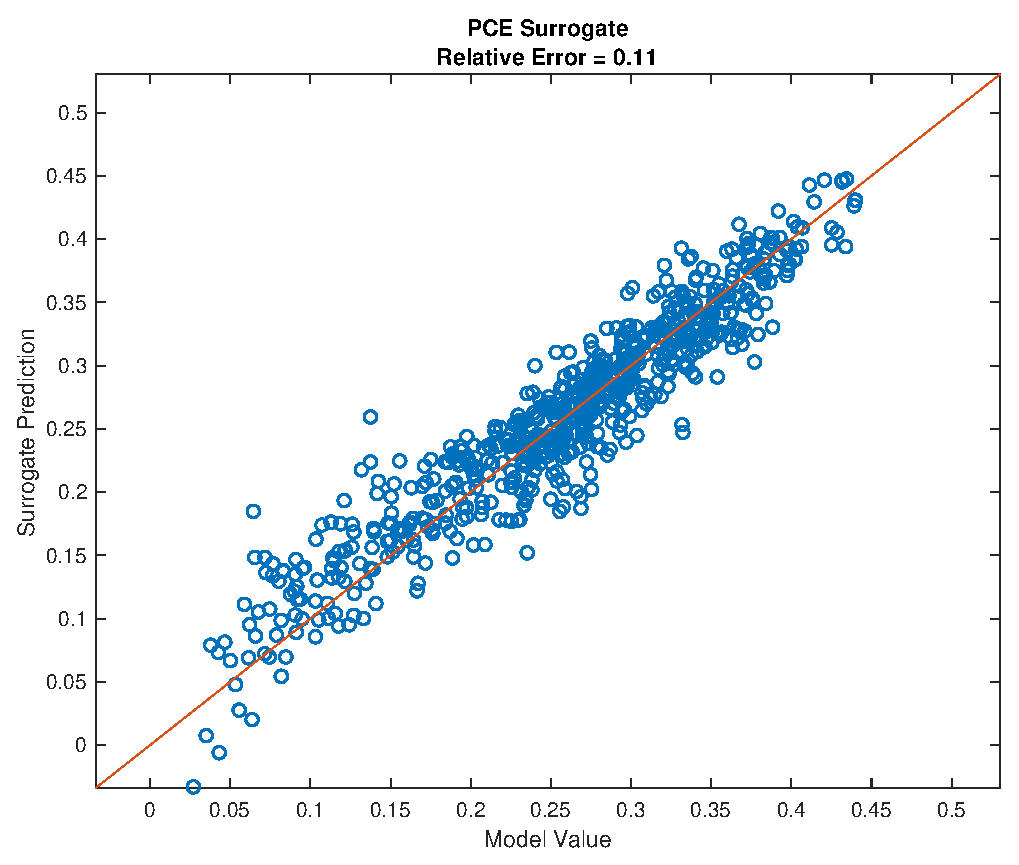
\includegraphics[width=.24 \textwidth]{Figures/AM_AMp_Min_QoI_PCE_Prediction_Rectangular.eps}
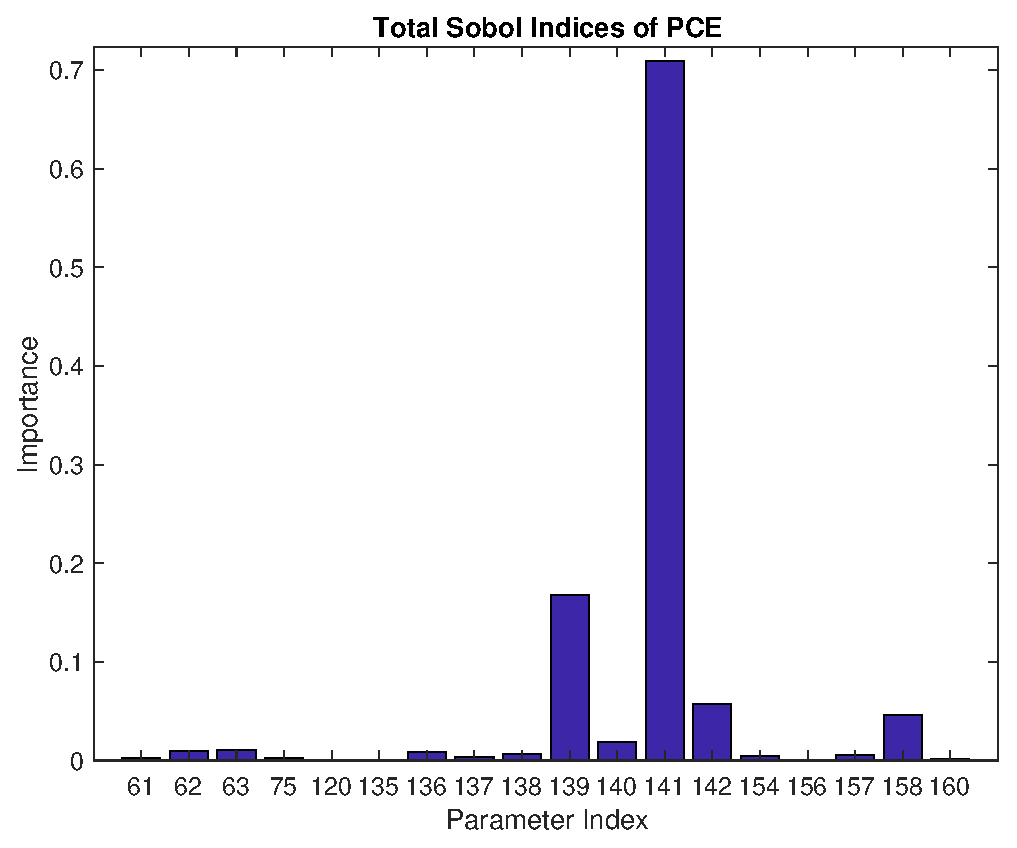
\includegraphics[width=.24 \textwidth]{Figures/AM_AMp_Min_QoI_PCE_SI_Rectangular.eps}\\
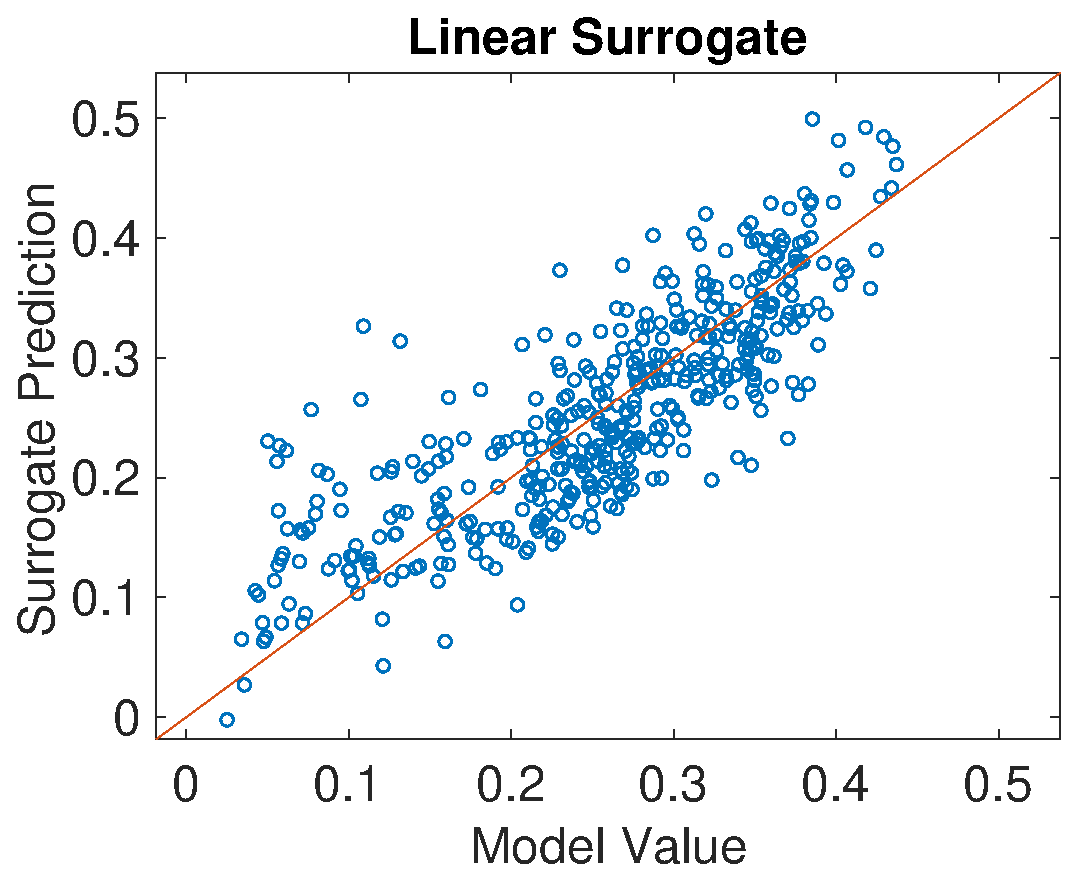
\includegraphics[width=.24 \textwidth]{Figures/AM_AMp_Min_QoI_LR_Prediction_Experimental.eps}
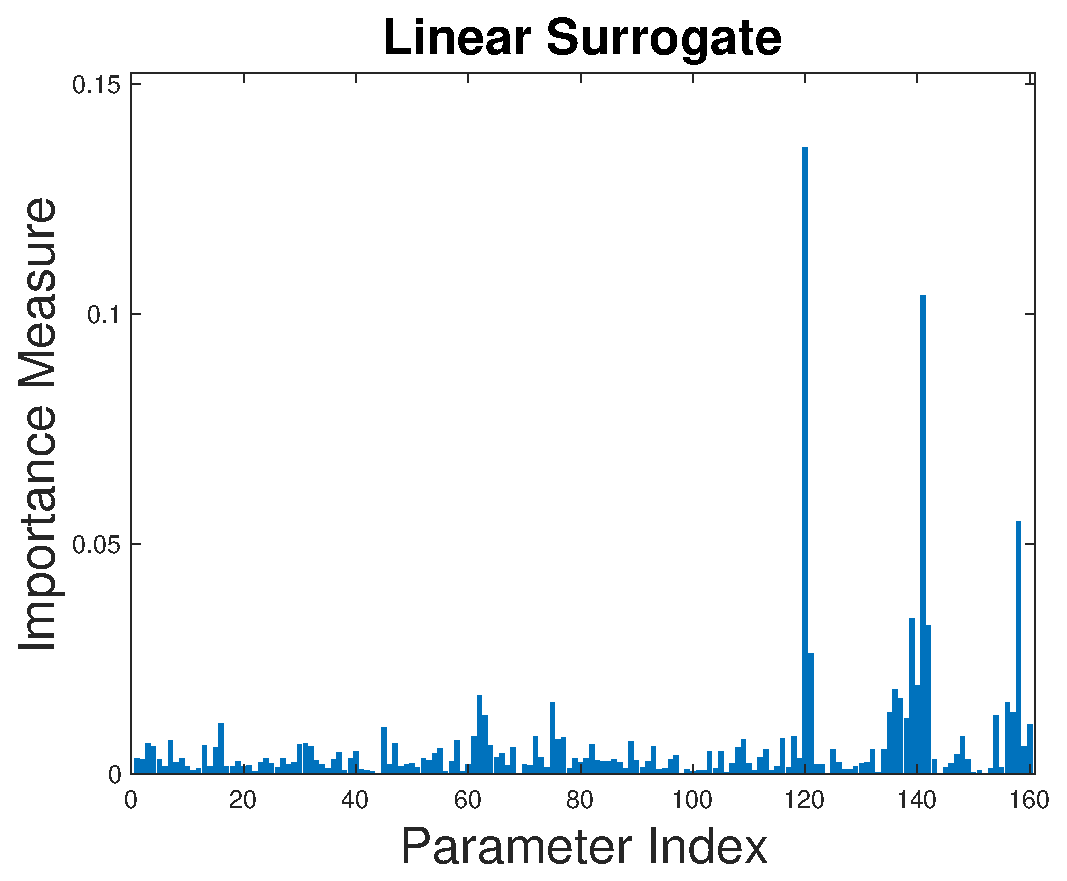
\includegraphics[width=.24 \textwidth]{Figures/AM_AMp_Min_QoI_LR_VI_Experimental.eps}
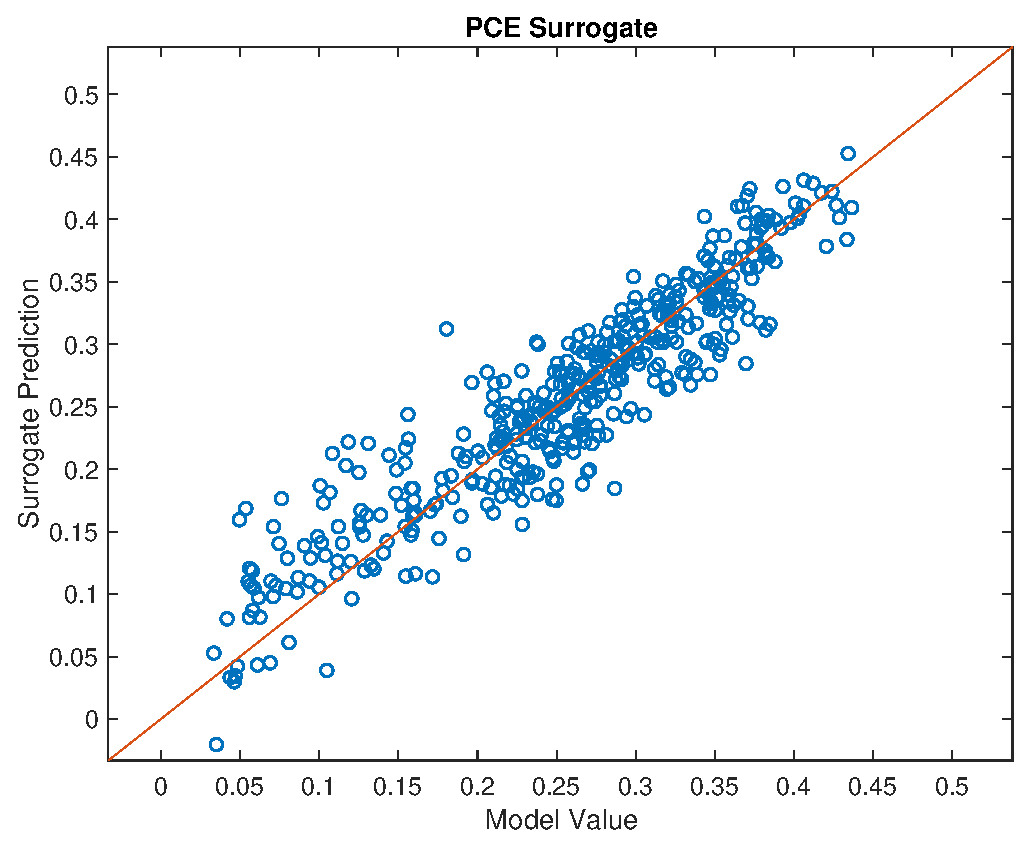
\includegraphics[width=.24 \textwidth]{Figures/AM_AMp_Min_QoI_PCE_Prediction_Experimental.eps}
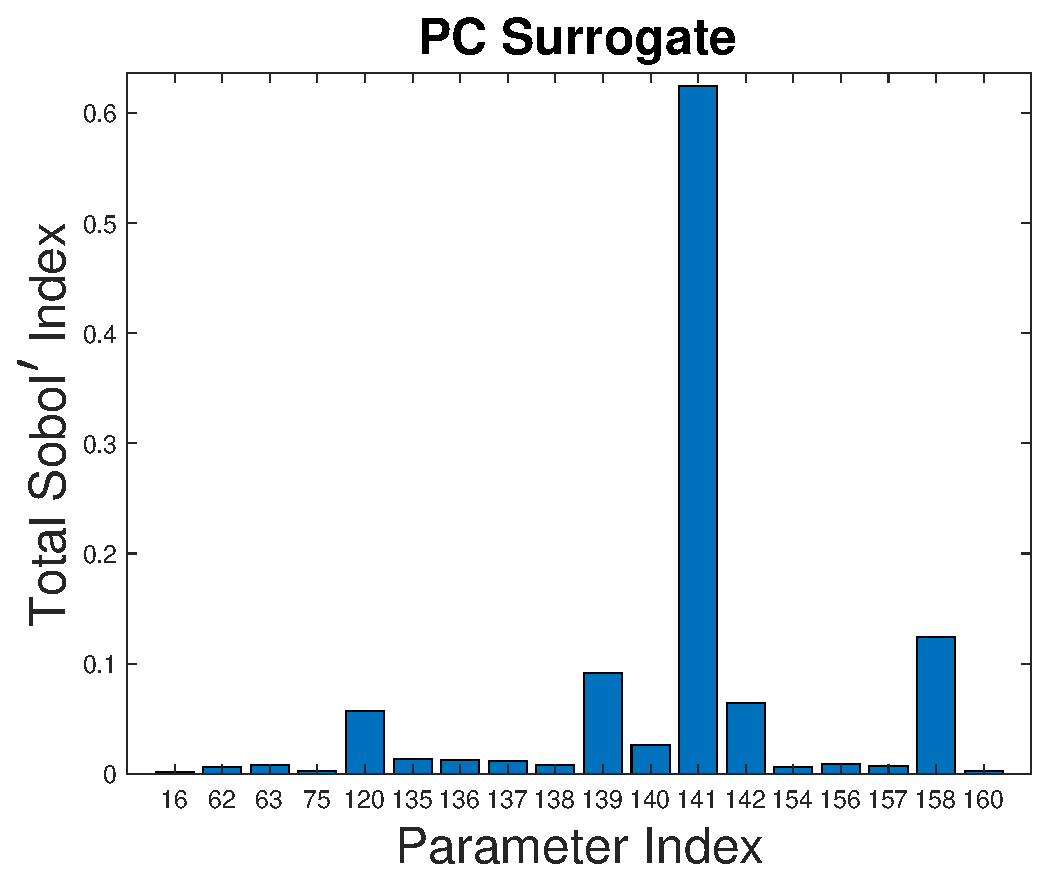
\includegraphics[width=.24 \textwidth]{Figures/AM_AMp_Min_QoI_PCE_SI_Experimental.eps}
\caption{Results for the minimum of the combined concentration of the actin myosin complex QoI. Top row: results with a rectangular pulse stimulus; bottom row: results with experimental data stimulus. From left to right, linear regression predictions, linear regression variable importance, PCE predictions, total Sobol' indices for PCE.}
\label{fig:qoi_AM_AMp_Min}
\end{figure}

The linear surrogate does not perform as well for this QoI; however, the PC surrogate is far more accurate; this highlights the nonlinearity of the QoI. The subset of parameters used in the PC surrogate differs for the rectangular pulse and experimental stimulus cases, but the most important parameters, as measured by the total Sobol' indices, agree. The most influential parameters for the minimum of the combined concentration of the actin myosin complex coincide with those for the volumetric flow rate in the cerebral tissue, an unsurprising result since both QoI are related to the wall mechanics. Parameter 120 appears important in the linear surrogate but unimportant in the PC surrogate.

\begin{table}[h]
\centering
\begin{tabular}{cccc}
Index & Identification & Total Sobol' Index (RP) & Total Sobol' Index (ES)\\
141 & z\_4 in SMCEC & 0.7095 & 0.6485\\
139 &  z\_2 in SMCEC & 0.1681 & 0.1465\\
142 & z\_5 in SMCEC & 0.0569 & 0.0341\\
158 & n\_cross in WallMechanics & 0.0463 & 0.0645\\
140 & z\_3 in SMCEC & 0.0189 & 0.0463\\
\end{tabular}
\caption{Most influential parameters for the combined concentration of the actin myosin complex QoI.}
\label{tab:qoi_AM_AMp_Min}
\end{table}

\section{Extra figures we probably won't include}
\subsection{$AM_p$ Time Lag}

\begin{figure}[h]
\centering
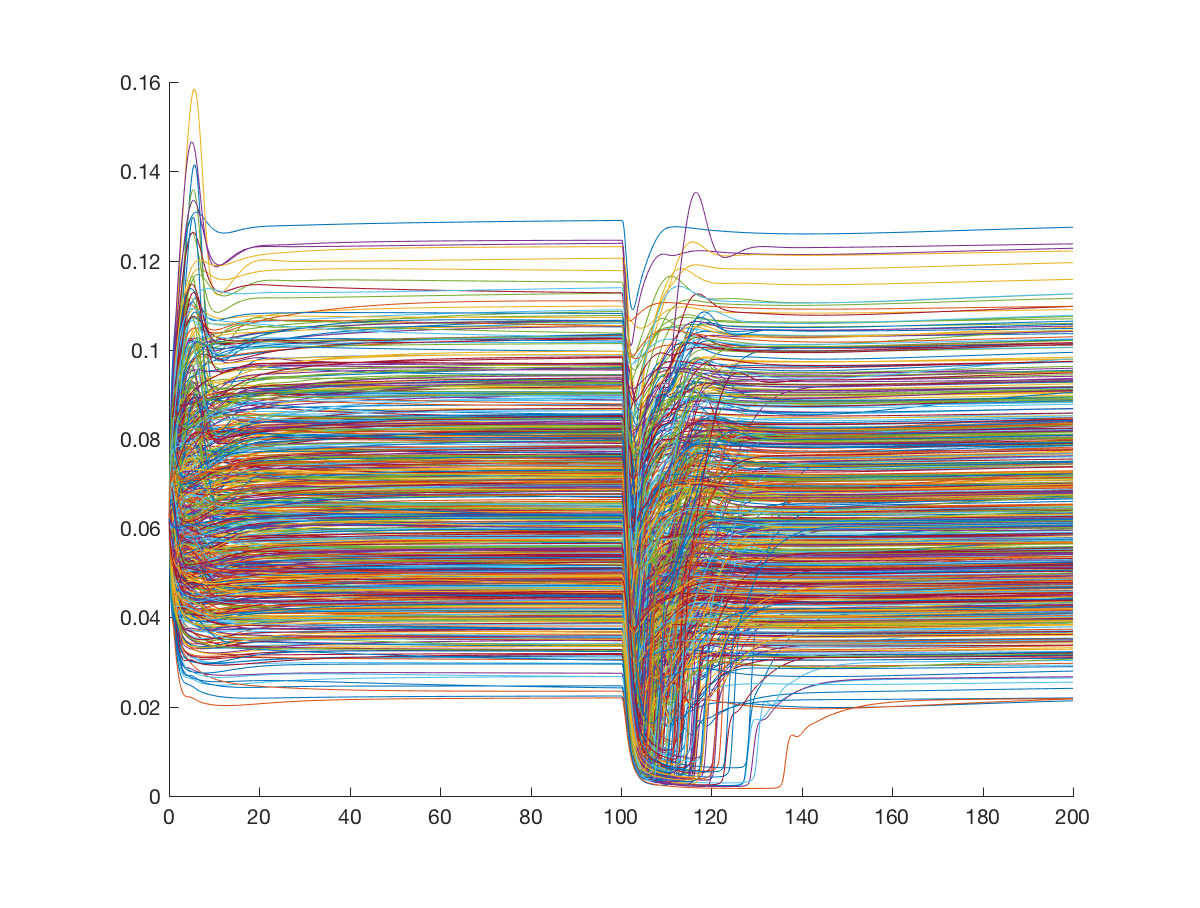
\includegraphics[width=.49 \textwidth]{Figures/AMp_Curves.eps}
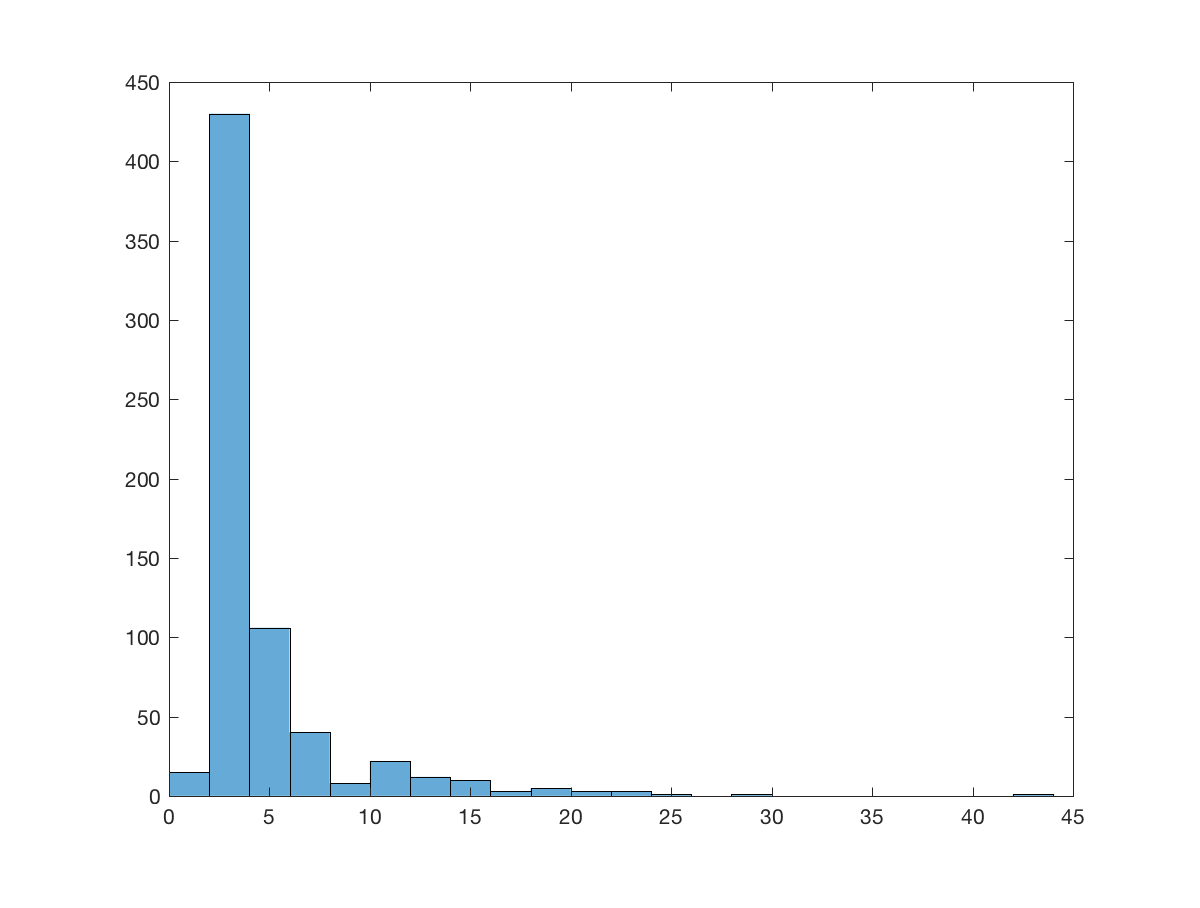
\includegraphics[width=.49 \textwidth]{Figures/AMp_Time_Lag_Histogram.eps}
\caption{$AM_p$ curves on the left and a histogram of the time lags on the right.}
\end{figure}

\subsection{Radius Time Lag}

\begin{figure}[h]
\centering
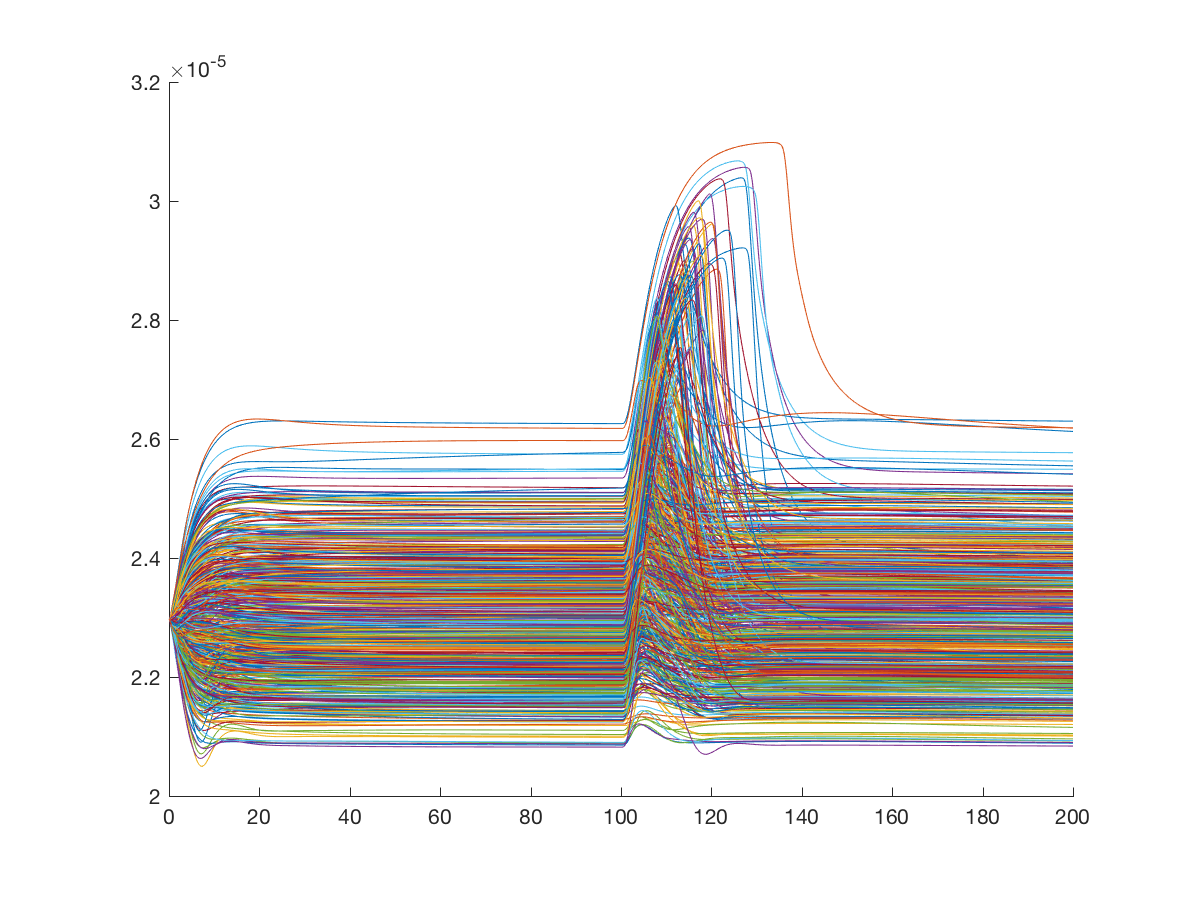
\includegraphics[width=.49 \textwidth]{Figures/Radius_Curves.eps}
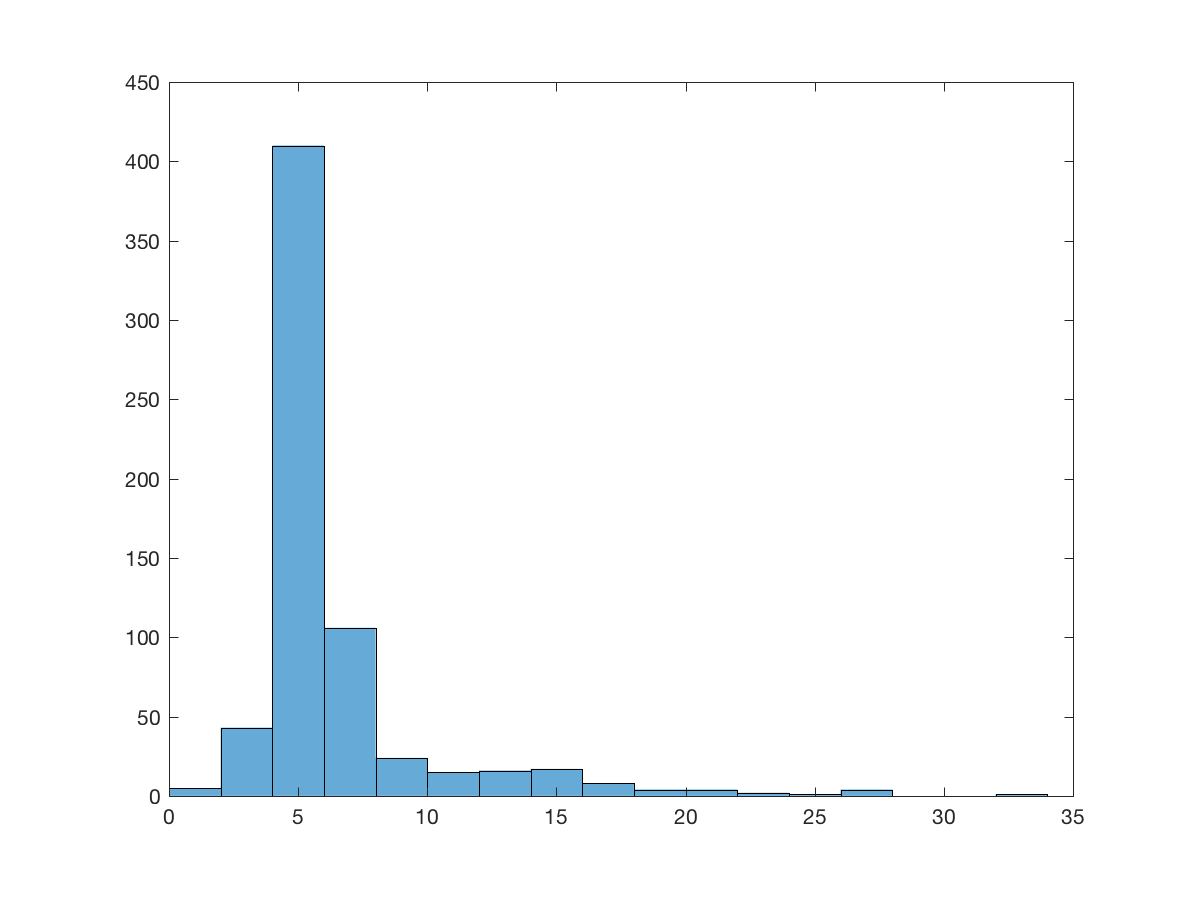
\includegraphics[width=.49 \textwidth]{Figures/Radius_Time_Lag_Histogram.eps}
\caption{Radius curves on the left and a histogram of the time lags on the right.}
\end{figure}

\section{Discussion}
ADD A DISCUSSION OF THE RESULTS IN TERMS OF THEIR PHYSIOLOGICAL INTERPRETATION

\section{Conclusion}
conclusion goes here

\bibliographystyle{KathisBibstyle} % no .sty!
\bibliography{library}

\end{document}